%
% chapter.tex -- Spezielle Funktionen definiert durch Integrale
%
% (c) 2021 Prof Dr Andreas Müller, Hochschule Rapperswil
%
% !TeX spellcheck = de_CH
\chapter{Integrale
\label{buch:chapter:integral}}
\lhead{Integrale}
\rhead{}
Der Analysis-Unterricht vermittelt manchmal den Eindruck, dass sich
für jede einigermassen anständige Funktion eine Stammfunktion
gefunden werden kann, wenn man nur genügend schlau ist und den 
nötigen Fleiss in die Lösung des Problems investiert.
Die Realität ist leider eine ganz andere, Ableiten ist zwar einfach,
eine Stammfunktion finden ist oft viel schwieriger und manchmal schlicht
unmöglich.

Der Ausweg aus dieser unangenehmen Situation ist, solche Integrale
als neue spezielle Funktionen zu definieren.
Eines der berühmtesten Beispiele für diesen Weg aus der Krise ist die
Fehlerfunktion, die im Abschnitt~\ref{buch:integrale:section:fehlerfunktion}
besprochen wird.
Auch geometrische Anwendungen führen auf solche Integrale.
Die Länge eines Ellipsenbogens kann mit Hilfe eines Integrals
berechnet werden, doch scheint es nicht möglich zu sein, für den
Umfang der Ellipse eine einfache Formel anzugeben, wie dies beim
Kreis möglich ist.
Dieses Problem führt auf eine ganze Familie von Integranden, die nicht in
geschlossener Form integriert werden können, nämlich die elliptischen
Funktionen.
Sie werden in Kapitel~\ref{buch:chapter:elliptischefunktionen} erklärt.

Doch wie entscheidet man, ob ein Integral tatsächlich nicht in geschlossener
Form dargestellt werden kann oder ob die Versuche einfach an mangelnden
eigenen Fähigkeiten gescheitert sind?
Denn warum soll man eine neue spezielle Funktion definieren, wenn es
dafür bereits eine gute Darstellung in geschlossener Form gibt?
Der Risch-Algorithmus von Abschnitt~\ref{buch:integral:section:risch}
gibt darauf eine Antwort.

%
% fehlerfunktion.tex
%
% (c) 2021 Prof Dr Andreas Müller, OST Ostschweizer Fachhochschule
%
\section{Die Fehlerfunktion
\label{buch:integrale:section:fehlerfunktion}}
\rhead{Fehlerfunktion}
Die Wahrscheinlichkeitsdichte einer normalverteilten Zufallsvariable $X$
mit Erwartungswert $\mu$ und Varianz $\sigma^2$ ist
\begin{equation}
\varphi(x)
=
\frac{1}{\sqrt{2\pi}\sigma}
e^{-\frac{(x-\mu)^2}{2\sigma^2}}.
\label{buch:integrale:eqn:normaldichte}
\end{equation}
Die Verteilungsfunktion der Zufallsvariable ist dann durch das Integral
\begin{equation}
f(x)
=
F_X(x)
=
P(X\le x)
=
\frac{1}{\sqrt{2\pi}\sigma}
\int_{-\infty}^x 
e^{-\frac{(t-\mu)^2}{2\sigma^2}}
\,dt
\label{buch:integrale:eqn:normalverteilung}
\end{equation}
gegeben.
Die Erfahrung zeigt, dass es sehr schwer ist, das
Integral~\eqref{buch:integrale:eqn:normalverteilung}
in geschlossener Form auszuwerten.
Die in Abschnitt~\ref{buch:integral:risch:subsection:liouville}
dargestellte Theorie von Liouville kann die Unmöglichkeit dieses
Unterfangens sogar beweisen.
Die Funktion $F_X(x)$ ist offenbar eine in Anwendungen nützliche und
häufig gebrauchte Funktion, die es verdient, in eine Standardbibliothek
von Funktionen aufgenommen zu werden.
Dabei soll auch berücksichtigt werden, dass die neu zu definierende
spezielle Funktion möglichst auch für andere Anwendungen verwendet
werden kann, wie zum Beispiel die Berechnung gewisser Laplace-Transformierter.
Im Folgenden soll gezeigt werden, in welcher Form genau dies geschehen
kann.

%
% Vereinfachung des Integrals durch Standardisierung
%
\subsection{Standardisierung}
Die Formel~\ref{buch:integrale:eqn:normalverteilung} enthält die zwei 
Parameter $\mu$ und $\sigma$, sie ist daher als Basis für eine neue
spezielle Funktion nicht geeignet.
In diesem Abschnitt sollen sie eliminiert werden mit dem Ziel, ein
neues, einfacheres Integral zu definieren, aus dem sich 
\ref{buch:integrale:eqn:normalverteilung} leicht berechnen lässt.

%
% Elimination der Parameter
%
\subsubsection{Elimination der Parameter $\mu$ und $\sigma$}
Aus der Wahrscheinlichkeitstheorie ist bekannt, dass zu einer
Zufallsvariablen $X$ mit Erwartungswert $E(X)=\mu$ und Varianz
$\operatorname{var}(X)=\sigma^2$ immer eine Zufallsvariable
gefunden werden kann mit Erwartungswert $0$ und Varianz $1$.
Tatsächlich bekommt man für die standardisierte Zufallsvariable
\begin{equation}
Z = \frac{X-\mu}{\sigma}
\label{buch:integrale:eqn:standardisierung}
\end{equation}
die Werte
\begin{align*}
E(Z)
&=
E\biggl(\frac{X-\mu}{\sigma}\biggr)
=
\frac{E(X)-\mu}{\sigma}
=
\frac{\mu-\mu}{\sigma}
=
0
\\
\text{und}\qquad
\operatorname{var}(Z)
&=
\operatorname{var}\biggl(\frac{X-\mu}{\sigma}\biggr)
=
\frac{\operatorname{var}(X)}{\sigma^2}
=
1,
\end{align*}
wie versprochen.
Dies bedeutet, dass sich das Integral~\ref{buch:integrale:eqn:normalverteilung}
durch ein Integral ausdrücken lassen muss, in der die Parameter $\mu$
und $\sigma$ nicht mehr vorkommen.

Die Standardisierungsformel~\eqref{buch:integrale:eqn:standardisierung}
deutet auch bereits an, wie man das
Integral~\ref{buch:integrale:eqn:normalverteilung} vereinfachen kann.
Dazu führen wir die Substitution $z=(t-\mu)/\sigma$ aus und erhalten
\begin{align*}
f(x)
&=
\frac{1}{\sqrt{2\pi}\sigma} 
\int_{-\infty}^x e^{-\frac{(t-\mu)^2}{2\sigma^2}}\,dt
=
\frac{1}{\sqrt{2\pi}\sigma}
\int_{\infty}^{(x-\mu)/\sigma}
e^{-\frac{z^2}2}\,\sigma dz
=
\frac{1}{\sqrt{2\pi}}
\int_{-\infty}^{\frac{x-\mu}{\sigma}} e^{-\frac{z^2}2}\,dz.
\end{align*}
Das Integral auf der rechten Seite enthält die Parameter $\mu$ und
$\sigma$ nur noch in der Integrationsgrenze.
Es kann durch die Wahrscheinlichkeitsverteilungsfunktion
\begin{equation}
\Phi(x) = \frac{1}{\sqrt{2\pi}} \int_{-\infty}^x e^{-\frac{z^2}2}\,dz
\label{buch:integrale:eqn:standardnormalverteilung}
\end{equation}
der Standardnormalverteilung als
\[
F_X(x) = \Phi\biggl(\frac{x-\mu}{\sigma}\biggr)
\]
ausgedrückt werden.
Die Funktion $\Phi(x)$ ist daher ein noch besserer Kandidat für eine
neue spezielle Funktion.

%
% Die Funktion erf(x)
%
\subsubsection{Die Funktion $\operatorname{erf}(x)$}
Die Funktion \eqref{buch:integrale:eqn:standardnormalverteilung} hat
einige Nachteile, die sich als Barriere für die numerische 
Berechnung der Funktionswerte herausstellen könnte.

Zunächst ist $\Phi(x)$ als ein uneigentliches Integral definiert.
Eine direkte numerische Integration muss daher über ein sehr grosses
Interval erstreckt werden, um die Genauigkeit garantieren zu können.
Jedoch ist bekannt, dass $\Phi(0)=\frac12$ ist, denn
\[
\Phi(0)
=
\frac{1}{\sqrt{2\pi}}
\int_{-\infty}^0 e^{-\frac{z^2}2}\,dz
=
\frac12\cdot\underbrace{\frac{1}{\sqrt{2\pi}}
\int_{-\infty}^{\infty} e^{-\frac{z^2}2}\,dz}_{\displaystyle=1}
=
\frac12.
\]
Man kann daher schreiben
\begin{equation}
\Phi(x) = \frac12 + \frac{1}{\sqrt{2\pi}}\int_0^x e^{-\frac{z^2}{z}}\,dz.
\label{buch:integrale:eqn:Phireduziert}
\end{equation}
Das Integral auf der rechten Seite ist ein gewöhnliches Integral und ist
damit viel einfacher zu berechnen.

Am Integral in~\eqref{buch:integrale:eqn:Phireduziert} ist aber immer
noch etwas unerfreulich, dass der Exponent komplizierter ist als nötig.
Mit Hilfe der Variablentransformation $u = z/\sqrt{2}$ erhalten wir
aus dem Integral in~\eqref{buch:integrale:eqn:Phireduziert}
\begin{align*}
\frac{1}{\sqrt{2\pi}}
\int_0^x e^{-\frac{z^2}2}\,dz
=
\frac{1}{\sqrt{2\pi}}
\int_0^{x/\sqrt{2}}
e^{-u^2} \, \sqrt{2}\,du
=
\frac{1}{\sqrt{\pi}}
\int_0^{x/\sqrt{2}}
e^{-u^2} \,du.
\end{align*}
Damit sind wir bei einer Funktion angekommen, die sich gut als spezielle
Funktion eignet.

\begin{definition}
Die {\em Fehlerfunktion} $\operatorname{erf}(x)$ ist die Funktion
\index{Fehlerfunktion}%
\index{erf(x)@$\operatorname{erf}(x)$}%
\[
\operatorname{erf}
\colon
\mathbb{R}\to [-1,1]
:
x
\mapsto
\operatorname{erf}(x)
:=
\frac{2}{\pi}
\int_0^x e^{-u^2}\,du.
\]
\end{definition}

\begin{figure}
\centering
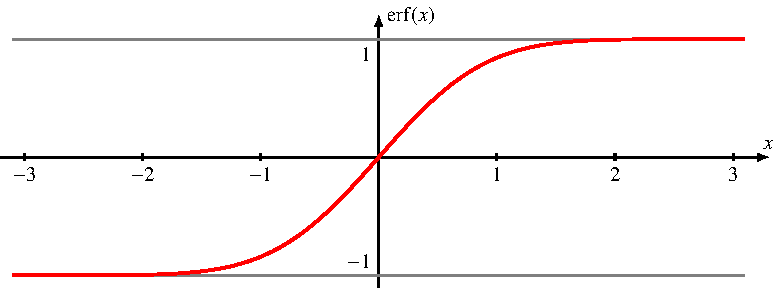
\includegraphics{chapters/060-integral/images/erf.pdf}
\caption{Graph der Fehlerfunktion $\operatorname{erf}(x)$
\label{buch:integrale:fig:erf}}
\end{figure}
Die Funktion $\operatorname{erf}$ nimmt Werte zwischen $-1$ und $1$ an,
wie man in Abbildung~\ref{buch:integrale:fig:erf} sehen kann.
Die horizontalen Geraden $y=\pm 1$ sind Asymptoten.
Die exakte Berechnung von $\operatorname{erf}(x)$ für sehr grosse Werte
des Argumentes gestaltet sich schwierig, da es zur starker Auslöschung
kommen kann.
Da die Funktionswerte $\operatorname{erf}(x)$ sehr nahe bei $1$ sind,
lohnt es sich, nicht $\operatorname{erf}(x)$, sondern $1-\operatorname{erf}(x)$
zu berechnen.

\begin{definition}
\index{komplementäre Fehlerfunktion}
\index{Fehlerfunktion, komplementäre}
\index{erfc(x)@$\operatorname{erfc}(x)$}
Die {\em komplementäre Fehlerfunktion} ist die Funktion
\[
\operatorname{erfc}
\colon
\mathbb{R} \to [0,2]
:
x\mapsto
\operatorname{erfc}(x)
:=
1-\operatorname{erf}(x)
=
\frac{2}{\sqrt{\pi}}\int_x^\infty e^{-u^2}\,du.
\]
Die {\em verallgemeinerte Fehlerfunktion} ist definiert als
\index{verallgemeinerte Fehlerfunktion}%
\index{Fehlerfunktion!verallgemeinerte}%
\index{erf(a,b)@$\operatorname{erf}(a,b)$}%
\[
\operatorname{erf}(a,b)
=
\frac{2}{\sqrt{\pi}}
\int_a^b e^{-u^2}\,du.
\]
\end{definition}

Mit der Fehlerfunktion kann die Standardnormalverteilungsfunktion jetzt
als
\[
\Phi(x)
=
\frac12
+
\frac12\operatorname{erf}\biggl( \frac{x}{\sqrt{2}} \biggr)
=
\frac12\biggl(
1+\operatorname{erf}\biggl(\frac{x}{\sqrt{2}}\biggr)\biggr)
\]
ausdrücken.
Die Verteilungsfunktion einer normalverteilten Zufallsvariable mit
Erwartungswert $\mu$ und Varianz $\sigma^2$ kann entsprechend mit
\[
F_X(x)
=
\frac12\biggl(
1+\operatorname{erf}\biggl(\frac{x-\mu}{\sqrt{2}\sigma}\biggr)
\biggr)
\]
berechnet werden.
Die Fehlerfunktion ist also eine ``gute'' spezielle Funktion, die
die Berechnung von Wahrscheinlichkeitswerten von normalverteilten
Zufallsvariablen vereinfacht.

%
% Fehlerfunktion als hypergeometrische Funktion
%
\subsubsection{Fehlerfunktion als hypergeometrische Funktion}
Die Fehlerfunktion ist eine Stammfunktion von
\[
\frac{2}{\sqrt{\pi}}
e^{-x^2}
=
\frac{2}{\sqrt{\pi}}
\biggl(
1 - \frac{x^2}{1!} + \frac{x^4}{2!} - \frac{x^6}{3!} + \frac{x^8}{4!}-\dots
\biggr).
\]
Durch gliedweises Integrieren erhält man
\begin{align}
\operatorname{erf}(x)
&=
\frac{2}{\sqrt{\pi}}
\biggl(
x - \frac{x^3}{1!\cdot 3} + \frac{x^5}{2!\cdot 5} - \frac{x^7}{3!\cdot 7} + \frac{x^9}{4!\cdot 9}-\dots
\biggr).
\notag
\intertext{Ein gemeinsamer Faktor $x$ kann ausgeklammert werden.
Die alternierenden Vorzeichen und die in Zweierschritten ansteigenden
Potenzen bedeuten, dass der Klammerausdruck als Reihe}
&=
\frac{2x}{\sqrt{\pi}}
\biggl(
1 +
\frac13\cdot\frac{(-x^2)^1}{1!}
+
\frac15\cdot\frac{(-x^2)^2}{2!}
+
\frac17\cdot\frac{(-x^2)^3}{3!}
+
\frac19\cdot\frac{(-x^2)^4}{4!}
+
\dots
+
\frac{1}{2k+1}\frac{(-x^2)^k}{k!}
+
\dots
\biggr)
\notag
\intertext{in $-x^2$ geschrieben werden kann.
Der Koeffzient $1/(2k+1)$ muss jetzt noch mit Pochhammer-Symbolen 
geschrieben werden.
Dazu wird er zunächst als $\frac12\cdot 1/(k+\frac12)$ geschrieben,
weil der Nenner dann in Einerschritten anwächst, wie dies für
Pochhammer-Symbole benötigt wird.
Das Pochhammer-Symbol $(\frac32)_k$ hat den korrekten letzten Faktor
$k+\frac12$, aber es hat viele zusätzliche Faktoren, nämlich
alle Faktoren in $(\frac12)_k$ ausser dem ersten.
Mit einem geeigneten Zähler können diese wieder zum Verschwinden
gebracht werden.
So erhält man die Darstellung
}
&=
\frac{2x}{\sqrt{\pi}}
\sum_{k=0}^\infty
\frac{1}{2\cdot (k+\frac12)}
\frac{(-x^2)^k}{k!}
=
\frac{2x}{\sqrt{\pi}}
\sum_{k=0}^\infty
\frac{1}{2} \cdot\frac{1}{k+\frac12}
\frac{(-x^2)^k}{k!}
\notag
\\
&=
\frac{2x}{\sqrt{\pi}}
\sum_{k=0}^\infty
\frac12
\cdot
\frac{
\frac32
\cdot \frac52
\cdot\ldots\cdot(k-\frac12)
\phantom{\mathstrut\cdot(k+\frac12)}
}{
\frac32
\cdot \frac52
\cdot\ldots\cdot(k-\frac12)\cdot(k+\frac12)
}
\frac{(-x^2)^k}{k!}
\notag
\\
&=
\frac{2x}{\sqrt{\pi}}
\sum_{k=0}^\infty
\frac{
\frac12
\cdot
\frac32
\cdot \frac52
\cdot\ldots\cdot(k-\frac12)
\phantom{\mathstrut\cdot(k+\frac12)}
}{
\phantom{\frac12\cdot\mathstrut}
\frac32
\cdot \frac52
\cdot\ldots\cdot(k-\frac12)\cdot(k+\frac12)
}
\frac{(-x^2)^k}{k!}
\notag
\\
&=
\frac{2x}{\sqrt{\pi}}
\sum_{k=0}^\infty \frac{(\frac12)_k}{(\frac32)_k}\frac{(-x^2)^k}{k!}
=
\frac{2x}{\sqrt{\pi}}
\,
\mathstrut_1F_1\biggl(
\begin{matrix}\frac12\\\frac32\end{matrix}; -x^2
\biggr)
\label{buch:integral:fehlerfunktion:eqn:alshypergeom}
\end{align}
der Fehlerfunktion als hypergeometrische Funktion.

%
% Laplace-Transformation der Fehlerfunktion
%
\subsection{Laplace-Transformation}
Wir berechnen die Laplace-Transformierte der Funktion
\[
f(t) = \operatorname{erf}\biggl(\frac{a}{2\sqrt{t}}\biggr).
\]
Nach Definition der Laplace-Transformation ist dies die Funktion
\begin{align*}
\mathscr{L}f(s)
&=
\int_0^\infty
e^{-st} \operatorname{erf}\biggl(\frac{a}{2\sqrt{t}}\biggr)
\,dt
=
\int_0^\infty
e^{-st}
\frac{2}{\sqrt{\pi}}
\int_0^{\frac{a}{2\sqrt{t}}}
e^{-x^2}
\,dx
\,dt.
\end{align*}
Das Integrationsgebiet $G$ ist der Teil des ersten Quadranten der
$t$-$x$-Ebene, für den die Ungleichung $x \le a/2\sqrt{t}$ gilt.
Dies ist gleichbedeutend mit $t \le a^2/4x^2$.
Vertauscht man die Integrationsreihenfolge, erhält man
\begin{align}
\mathscr{L}f(s)
&=
\int_G
e^{-st}
\frac{2}{\sqrt{\pi}}
e^{-x^2}
\,dx \,dt
=
\int_0^\infty
\int_0^{\frac{a^2}{4x^2}}
e^{-st}
\frac{2}{\sqrt{\pi}}
e^{-x^2}
\,dt
\,dx
=
\frac{2}{\sqrt{\pi}}
\int_0^\infty
e^{-x^2}
\int_0^{\frac{a^2}{4x^2}}
e^{-st}
\,dt
\,dx
\notag
\\
&=
\frac{2}{\sqrt{\pi}}
\int_0^\infty
e^{-x^2}
\biggl[
-\frac1{s}e^{-st}
\biggr]_0^{\frac{a^2}{4x^2}}
\,dx
=
\frac{2}{\sqrt{\pi}}
\int_0^\infty
e^{-x^2}
\frac1{s}
\biggl(
1-e^{-\frac{sa^2}{4x^2}}
\biggr)
\,dx
\notag
\\
&=
\frac{1}{s}
\cdot
\frac{2}{\sqrt{\pi}}\int_0^\infty e^{-x^2}\,dx
-
\frac1{s}
\cdot
\frac{2}{\sqrt{\pi}}
\int_0^\infty
e^{-x^2-\frac{sa^2}{4x^2}}
\,dx
\notag
\\
&=
\frac1s\lim_{x\to\infty} \operatorname{erf}(x)
-
\frac1s
\cdot
\frac{2}{\sqrt{\pi}}
\int_0^\infty e^{-\left(x^2+\frac{sa^2}{4x^2}\right)}\,dx.
\label{buch:integrale:eqn:laplaceerf}
\end{align}
Der Grenzwert im ersten Term ist $1$, nach Definition der Fehlerfunktion. 
Schreiben wir $b=a\sqrt{s}/2$, dann wird das Integral im zweiten Term
\begin{equation}
I(b)
=
\int_0^\infty e^{-\left(x^2+\frac{sa^2}{4x^2}\right)}\,dx
=
\int_0^\infty \exp\biggl(-\biggl(x^2+\frac{b^2}{x^2}\biggr)\biggr)\,dx.
\label{buch:integrale:eqn:Ibsumme}
\end{equation}
Den Exponenten im Integranden kann man wie folgt als quadratischen
Ausdruck in $x\pm a/x$ schreiben:
\begin{equation*}
\begin{aligned}
%\biggl(
x^2 + \frac{b^2}{x^2}
%\biggr)
&=
\biggl(x+\frac{b}{x}\biggr)^2 - 2b
\\
&=
\biggl(x-\frac{b}{x}\biggr)^2 + 2b.
\end{aligned}
\end{equation*}
Man kann also das Integral $I(b)$ auf die eine oder andere Art als
\begin{equation}
\begin{aligned}
I(b)
&=
\int_0^\infty \exp\biggl(-\biggl(x+\frac{b}{x}\biggr)^2+2b\biggr)\,dx
\\
\text{oder}\quad\phantom{I(b)}
&=
\int_0^\infty \exp\biggl(-\biggl(x-\frac{b}{x}\biggr)^2-2b\biggr)\,dx
\end{aligned}
\label{buch:integrale:eqn:fehlerintegrale}
\end{equation}
schreiben.
Die Faktoren $e^{\pm 2b}$ können aus dem Integral genommen werden.
Trotzdem kann man das Integral nicht einfach ausführen.

Die Substitution $y=x\pm\frac{b}{x}$ vereinfacht den Integranden
\eqref{buch:integrale:eqn:fehlerintegrale}
zwar zu $e^{-y^2}$, aber die Substitution für $dx$ liefert
\begin{equation}
y=x\pm\frac{b}{x}
\qquad\Rightarrow\qquad
dy = \biggl(1\mp \frac{b}{x^2}\biggr)\,dx.
\label{buch:integrale:eqn:dy}
\end{equation}
Dies kann für die Berechnung von $I(b)$ verwendet werden.
Zunächst folgt aus \eqref{buch:integrale:eqn:fehlerintegrale},
dass jede konvexe Kombination der beiden Integrale mit Koeffizienten,
die sich zu $1$ summieren, wieder $I(b)$ ergibt.
Wählen wir die Koeffizienten 
\[
\frac12\biggl(1\mp\frac{b}{x^2}\biggr),
\]
dann heben sich die Terme mit $b/x^2$ weg, wir erhalten die
konvexe Kombination
\[
I(b)
=
\frac12
\cdot
\underbrace{
\int_0^\infty
\biggl(1-\frac{b}{x^2}\biggr)
\exp\biggl(-\biggl(x+\frac{b}{x}\biggr)^2\biggr)\,dx
}_{\displaystyle=I_+(b)}
\mathstrut
\cdot e^{2b}
+
\frac12
\underbrace{
\int_0^\infty
\biggl(1+\frac{b}{x^2}\biggr)
\exp\biggl(-\biggl(x-\frac{b}{x}\biggr)^2\biggr)\,dx
}_{\displaystyle=I_-(b)}
\mathstrut
\cdot e^{-2b},
\]
die aus zwei Integralen besteht, die einfacher berechnet werden können.

Im Integral $I_-(b)$ können wir die Substitution \eqref{buch:integrale:eqn:dy}
ausführen
und erhalten
\begin{align*}
I_-(b)
&=
\int_{-\infty}^\infty
\biggl(1+\frac{b}{x^2}\biggr)
\exp\biggl(-\biggl(x-\frac{b}{x}\biggr)^2\biggr)\,dx
=
\int_{-\infty}^\infty e^{-y^2}\,dy
=
\frac{\sqrt{\pi}}2
\end{align*}
nach Definition der Fehlerfunktion.

Das erste Integral $I_+(b)$ ist etwas schwieriger zu berechnen.
Die Substition $z=b/x$ bildet das Integrationsinterval auf sich selbst ab,
aber die Integrationsrichtung kehrt um.
Mit
\[
dz = -\frac{b}{x^2}\,dx
\qquad\Rightarrow\qquad
dx = -\frac{z^2}{b}\,dz
\]
erhalten wir jetzt
\begin{align*}
I_+(b)
&=
\int_0^\infty
\biggl(1-\frac{b}{x^2}\biggr)
\exp\biggl(-\biggl(x+\frac{b}{x}\biggr)^2\biggr)\,dx
\\
&=
\int_{\infty}^0
\biggl(1-\frac{b}{b^2/z^2}\biggr)
\exp\biggl(-\biggl(\frac{b}{z}+z\biggr)^2\biggr)\,
\biggl(-\frac{b}{z^2}\biggr)\,dz
\\
&=
\int_{0}^{\infty}
\biggl(1-\frac{b}{b^2/z^2}\biggr)
\exp\biggl(-\biggl(\frac{b}{z}+z\biggr)^2\biggr)\,
\frac{b}{z^2}\,dz
\\
&=
\int_{0}^{\infty}
\biggl(\frac{b}{z^2}-1\biggr)
\exp\biggl(-\biggl(\frac{b}{z}+z\biggr)^2\biggr)\,
dz
=
-I_+(b).
\end{align*}
Indem man auf beiden Seiten $I_+(b)$ addiert erhält man nun $2I_+(b)=0$,
also auch $I_+(b)=0$.
Das Integral $I_+(b)$ verschwindet also, $I_+(b)=0$.

Nach all diesen Zwischenrechnungen können wir jetzt das Integral $I(b)$
zusammensetzen.
Wir finden
\begin{align*}
I(b)
&=
\frac12e^{2b} I_+(b) +\frac12e^{-2b} I_-(b)
\\
&=
\frac12e^{-a\sqrt{s}}\cdot \frac{\sqrt{\pi}}{2}.
\end{align*}
Einsetzen in \eqref{buch:integrale:eqn:laplaceerf} gibt jetzt das
Resultat für die Laplace-Transformierte von $f(t)$, sie ist
\[
\mathscr{L}f(s)
=
\frac1s - \frac1s\cdot\frac{2}{\sqrt{\pi}} I(b)
=
\frac1s\biggl(1-\frac12e^{-a\sqrt{s}} \biggr).
\]

\begin{satz}
\index{Satz!Laplace-Transformierte der Fehlerfunktion}%
Die Laplace-Transformierte der Fehlerfunktion mit Argument
$a/2\sqrt{t}$ ist
\begin{equation}
f(t) = \operatorname{erf}\biggl(\frac{a}{2\sqrt{t}}\biggr)
\qquad\multimapdotbothA\qquad
\mathscr{L}f(s)
=
\frac1s\biggl(1-\frac12e^{-a\sqrt{s}}\biggr).
\end{equation}
\end{satz}




\subsection{Berechnungsmethoden}
Die Fehlerfunktion kann natürlich mit numerischen Integrationsmethoden
berechnet werden.
Diese verlangen jedoch typischerweise die Auswertung des Integranden
an einer grossen Zahl von Stützstellen.
Im vorliegenden Falle müsste die transzendente Exponentialfunktion
sehr häufig berechnet werden, was zu sehr langer Laufzeit führt.
Gefragt sind daher Berechnungsverfahren, die möglichst nur arithmetische
Operationen verwenden, die sehr schnell in Hardware ausgeführt werden
können.

\subsubsection{Taylorreihe}
Die Fehlerfunktion ist das Integral einer Exponentialfunktion, die mit
Hilfe einer Potenzreihe für beliebige Argumente berechnet werden kann.
Aus
\[
e^x
=
1+x+\frac{x^2}{2!}+\frac{x^3}{3!} + \dots
=
\sum_{k=0}^\infty \frac{x^k}{k!}
\]
erhalten wir die Potenzreihe
\begin{equation}
e^{-t^2}
=
\sum_{k=0}^{\infty}
(-1)^k
\frac{t^{2k}}{k!},
\label{buch:integrale:eqn:erftaylor}
\end{equation}
die für alle Werte von $t$ konvergiert.

Da die Reihe
\eqref{buch:integrale:eqn:erftaylor}
absolut konvergiert, darf man sie gliedweise integrieren und erhält
\begin{equation}
\operatorname{erf}(x)
=
\frac{2}{\sqrt{\pi}}
\int_0^x
e^{-t^2}\,dt
=
\frac{2}{\sqrt{\pi}}
\sum_{k=0}^\infty \frac{(-1)^k}{k!}\int_0^x t^{2k}\,dt
=
\frac{2}{\sqrt{\pi}}
\sum_{k=0}^\infty \frac{(-1)^kx^{2k+1}}{k!(2k+1)}.
\label{buch:integrale:eqn:erfreihe}
\end{equation}
Diese Reihenentwicklung ist sehr effizient für kleine Werte von $x$.
Für grosse Werte von $x$ entstehen aber sehr grosse Zwischenterme in der
Reihe, was zu Auslöschung und damit zu Genauigkeitsverlust führt.

\subsubsection{Hypergeometrische Funktion}
Die in \eqref{buch:integral:risch:subsection:liouville}
gefundene Darstellung

%Die Taylor-Reihe~\eqref{buch:integrale:eqn:erfreihe} der Fehlerfunktion
%kann auch mit Hilfe hypergeometrischer Funktionen geschrieben werden.
%Da nur ungerade Potenzen vorkommen, klammern wir zunächst einen gemeinsamen
%Faktor $x$ aus:
%\[
%\operatorname{erf}(x)
%=
%\frac{2x}{\sqrt{\pi}}
%\sum_{k=0}^\infty
%\frac{1}{2k+1}
%\frac{(-x^2)^k}{k!}.
%\]
%Der Bruch $1/(2k+1)$  muss jetzt noch mit Hilfe von Pochhammer-Symbolen
%geschrieben werden.
%Dazu beachten wir, dass
%\begin{align*}
%\frac{1}{2k+1} 
%&=
%\frac12
%\frac{1}{\frac32+k-1}
%\\
%&=
%\frac12
%\frac{
%\frac32(\frac32+1)(\frac32+2)\dots(\frac32+k-2)\phantom{(\frac32+k-1)}
%}{
%\frac32(\frac32+1)(\frac32+2)\dots(\frac32+k-2)(\frac32+k-1)
%}
%\\
%&=
%\frac{
%\frac12(\frac12+1)(\frac12+2)(\frac12+3)\dots(\frac12+k-1)
%}{
%\frac32(\frac32+1)(\frac32+2)\dots(\frac32+k-2)(\frac32+k-1)
%}
%\\
%&=
%\frac{(\frac12)_k}{(\frac32)_k}.
%\end{align*}
%Somit ist die Fehlerfunktion als hypergeometrische Funktion
\[
\operatorname{erf}(x)
=
\frac{2x}{\sqrt{\pi}}\sum_{k=0}^\infty
\frac{(\frac12)_k}{(\frac32)_k}\frac{(-x^2)^k}{k!}
=
\frac{2x}{\sqrt{\pi}}\,
\mathstrut_1F_1\biggl(\begin{matrix}{\textstyle\frac12}\\{\textstyle\frac32}\end{matrix};-x^2\biggr).
\]
als hypergeometrische Reihe erlaubt, $\operatorname{erfc}(x)$
direkt zu berechnen.

%
% Kettenbruchentwicklung
%
\subsubsection{Kettenbruchentwicklung}
Besonders für grosse $x$ interessiert man sich mehr für
$\operatorname{erfc}(x)$ als für $\operatorname{erf}(x)$.
Die Potenzreihe \eqref{buch:integrale:eqn:erfreihe} ist
dafür wegen der bereits erwähnten Auslöschung besonders ungeeignet.
Man kann aber die Kettenbruchentwicklung 
\begin{equation}
\operatorname{erfc}(z)
=
\frac{2ze^{-z^2}}{\sqrt{\pi}}
\cfrac{1}{
z+\cfrac{\frac12}{
z+\cfrac{\frac22}{
z+\cfrac{\frac32}{
z+\cfrac{\frac42}{
z+\cfrac{\frac52}{
z+\cfrac{\frac62}{
z+\dots}}}}}}}
\end{equation}
finden, die in \cite[p.~175]{buch:pade} dargestellt wird.
Für grosse $z$ liefert dieser Kettenbruch besonders schnell konvergierende
Näherungsbrüche für $\operatorname{erfc}(z)$.

Das Kapitel~\ref{chapter:0f1} enthält weiter Informationen zu
den Zusammenhängen zwischen hypergeometrischen Funktionen und
Kettenbrüchen.

%
% Interpolation
%
\subsubsection{Interpolation}
Die GNU Scientific Library \cite{buch:library:gsl} verwendet eine Reihe von
Tschebyscheff-Approximationspolynomen, die für die Intervalle, in denen
sie definiert sind, besonders effizient zu berechnende Approximation
mit Maschinengenauigkeit ergeben.

%
% eulertransformation.tex
%
% (c) 2021 Prof Dr Andreas Müller, OST Ostschweizer Fachhochschule
%
\section{Integraleigenschaften hypergeometrischer Funktionen
\label{buch:integral:section:eulertransformation}}
\rhead{Euler-Transformation}
Die hypergeometrischen Funktionen wurden bisher einerseits
als Reihen mit einer speziellen Rekursionsrelation der Reihenglieder
und als Lösungen einer speziellen Art von Differentialgleichung
erkannt.
In diesem Abschnitt soll untersucht werden, ob man sie auch
auch durch Integrale definieren kann.

%
% Integraldarstellung der hypergeometrischen Funktion 2F1
%
\subsection{Integraldarstellung der hypergeometrischen Funktion
$\mathstrut_2F_1$}
Das Integral
\[
f(x)
=
\int_0^1 t^{b-1} (1-t)^{c-b-1} (1-xt)^{-a}\,dt
\]
kann im Allgemeinen nicht in geschlossener Form evaluiert werden.
Es wäre daher naheliegend, es als neues spezielle Funktion zu definieren.
Die folgende Rechnung soll aber zeigen, dass es sich durch die bereits
bekannte hypergeometrische Fujnktion $\mathstrut_2F_1$ ausdrücken
lässt.

Die Newtonsche binomische Reihe ermöglicht, den $x$ enthaltenden
Faktor als
\[
(1-xt)^{-a}
=
\sum_{k=0}^\infty
\frac{(a)_k}{k!} x^k t^k
\]
zu schreiben.
Setzt man dies ins Integral ein, erhält man
\[
f(x)
=
\sum_{k=0}^\infty \frac{(a)_k}{k!} x^k
\int_0^1 t^{b-1} (1-t)^{c-b-1} t^k\,dt
=
\sum_{k=0}^\infty \frac{(a)_k}{k!} x^k
\int_0^1 t^{k+b-1} (1-t)^{c-b-1}\,dt.
\]
Das Integral ist die Beta-Funktion $B(k+b,c-b)$ und kann daher mit Hilfe
der Gamma-Funktion geschrieben werden.
Es gilt
\[
B(k+b,c-b)
=
\frac{\Gamma(k+b)\Gamma(c-b)}{\Gamma(c+k)}.
\]
Mit Hilfe der Funktionalgleichung der Gamma-Funktion kann man
\begin{align*}
\Gamma(u+k)
&=
\Gamma(u+k-1) (u+k-1)
=
\Gamma(u+k-2) (u+k-2)(u+k-1)
\\
&=
\ldots
\\
&=
\Gamma(u) u(u+1)\cdots(u+k-2)(u+k-1)
\end{align*}
schreiben, womit das Integral zu
\begin{align*}
f(x)
&=
\sum_{k=0}^\infty \frac{(a)_k}{k!} x^k
\frac{\Gamma(k+b)\Gamma(c-b)}{\Gamma(c+k)}
=
\sum_{k=0}^\infty \frac{(a)_k}{k!} x^k
\frac{\Gamma(b)(b)_k\Gamma(c-b)}{\Gamma(c)(c)_k}
\\
&=
\frac{\Gamma(b)\Gamma(c-b)}{\Gamma(c)}
\sum_{k=0}^\infty\frac{(a)_k(b)_k}{(c)_k} x^k
=
\frac{\Gamma(b)\Gamma(c-b)}{\Gamma(c)}\,
\mathstrut_2F_1\biggl(\begin{matrix}a,b\\c\end{matrix};x\biggr)
\end{align*}
vereinfacht werden kann.
Damit ist das Integral bestimmt. 
Durch Auflösung nach der hypergeometrischen Funktion bekommt man
die folgende Integraldarstellung.

\begin{satz}[Euler]
\index{Satz!Eulertransformation}%
\label{buch:integrale:eulertransformation:satz}
Die hypergeometrische Funktion $\mathstrut_2F_1$ kann durch das 
Integral
\begin{equation}
\mathstrut_2F_1\biggl(\begin{matrix}a,b\\c\end{matrix};z\biggr)
=
\frac{\Gamma(c)}{\Gamma(b)\Gamma(c-b)}
\int_0^1
t^{b-1}(1-t)^{c-b-1}(1-zt)^{-a}
\,dt
\label{buch:integrale:eulertransformation:satzeqn}
\end{equation}
dargestellt werden.
\end{satz}

%
% Alternative Parametrisierungen
%
\subsubsection{Alternative Parametrisierungen}
Die Substitution $t=\sin^2 s$ ermöglicht eine alternative Parametrisierung
der Integraldarstellung der hypergeometrischen Funktion.
Wenden wir sie auf~\eqref{buch:integrale:eulertransformation:satzeqn}
an, erhalten wir wegen $dt = 2\cos s\sin s\,ds$
\begin{align*}
\mathstrut_2F_1\biggl(\begin{matrix}a,b\\c\end{matrix};z\biggr)
&=
\frac{\Gamma(c)}{\Gamma(b)\Gamma(c-b)}
\int_0^{\frac{\pi}2}
\sin^{2(b-1)}(s)\,
(1-\sin^2s)^{c-b-1} (1-z\sin^2 s)^{-a}
\,\cos s\sin s
\,ds
\\
&=
\frac{\Gamma(c)}{\Gamma(b)\Gamma(c-b)}
\int_0^{\frac{\pi}2}
\sin^{2b-1}(s)\,\cos^{2c-2b-1}(s)\, (1-z\sin^2 s)^{-a}
\,ds.
\end{align*}

Die Substitution $t=s/(s+1)$ wird das Integral zu einem Integral
über $[0,\infty)$
\begin{align*}
\mathstrut_2F_1\biggl(\begin{matrix}a,b\\c\end{matrix};z\biggr)
&=
\frac{\Gamma(c)}{\Gamma(b)\Gamma(c-b)}
\int_0^1
\biggl(\frac{s}{s+1}\biggr)^{b-1}
\biggl(\frac{1}{s+1}\biggr)^{c-b-1}
\biggl(\frac{1+s-zs}{s+1}\biggr)^{-a}
\,dt
\\
&=
\frac{\Gamma(c)}{\Gamma(b)\Gamma(c-b)}
\int_0^1
\frac{
s^{b-1}
}{
(s+1)^{c-a}
}
(1+s-zs)^{-a}
\,dt.
\end{align*}

%
% Integraldarstellung asl Integraltransformation
%
\subsection{Integraldarstellung als Integraltransformation}
Im vorangegangenen Abschnitt wurde gezeigt, wie sich die Funktion
$\mathstrut_2F_1$ als ein Integral des Integranden
\[
t^{b-1}(1-t)^{c-b-1} (1-xt)^{-a}
\]
ausdrücken lässt.
Der letzte Faktor $(1-xt)^{-a}$ kann mit der Binomialreihe
\begin{align*}
(1+x)^\alpha
&=
1
+ 
\alpha x
+
\frac{\alpha(\alpha-1)}{2!}x^2
+
\frac{\alpha(\alpha-1)(\alpha-2)}{3!}x^3
+
\cdots
\\
&=
1
+
\frac{-\alpha}{1}(-x)
+
\frac{-\alpha(-\alpha+1)}{2!} (-x)^2
+
\frac{-\alpha(-\alpha+1)(-\alpha+2)}{3!} (-x)^3
+
\cdots
\\
&=
\sum_{k=0}^\infty \frac{(-\alpha)_k}{k!} (-x)^k
=
\mathstrut_0F_1\biggl(
\begin{matrix}
\text{---}\\-\alpha
\end{matrix}
;-x
\biggr)
\end{align*}
als hypergeometrische Funktion geschrieben werden.
Die Integraldarstellung von $\mathstrut_2F_1$ kann daher auch 
in die Form
\begin{equation}
\mathstrut_2F_1\biggl(\begin{matrix}a,b\\c\end{matrix};z\biggr)
=
\frac{\Gamma(c)}{\Gamma(b)\Gamma(c-b)}
\int_0^1 t^{b-1}(1-t)^{c-b-1}
\,
\mathstrut_0F_1(;a;zt)\,dt
\label{buch:integral:eqn:trafovorstufe}
\end{equation}
umgeformt werden.

Eine gewisse Ähnlichkeit zur Laplace-Transformation ist der
Formel~\eqref{buch:integral:eqn:trafovorstufe} nicht abzusprechen.
Die Funktion \( t^{b-1}(1-t)^{c-b-1} \) wird statt mit der
Exponentialfunktion $e^{xt} = \mathstrut_0F_0(xt)$ mit der
hypergeometrischen Funktion $\mathstrut_0F_1(;a;xt)$ multipliziert und
integriert.
Dies suggeriert, dass sich möglicherweise jede der hypergeometrischen
Funktionen $\mathstrut_{p+1}F_{q+1}$ durch ein Integral, dessen 
Integrand $\mathstrut_pF_q$ enthält, ausdrücken lässt.

\begin{satz}
\index{Satz!Euler-Transformationformel}%
Es gilt die sogennannte {\em Euler-Transformationsformel}
\index{Euler-Transformation}%
\[
\mathstrut_{p+1}F_{q+1}\biggl(
\begin{matrix}
a_1,\dots,a_{p+1}\\
b_1,\dots,b_{q+1}
\end{matrix}
;z
\biggr)
=
\frac{\Gamma(b_{q+1})}{\Gamma(a_{p+1})\Gamma(b_{q-1}-a_{p+1})}
\int_0^1
t^{a_{p+1}-1}(1-t)^{b_{q+1}-a_{p+1}-1}
\mathstrut_pF_q\biggl(
\begin{matrix}
a_1,\dots,a_p\\
b_1,\dots,b_q
\end{matrix};zt
\biggr)
\,dt.
\]
\end{satz}

\begin{proof}[Beweis]
Sei $I$ das Integral auf der rechten Seite.
Wir setzen die Reihenentwicklung der Funktion $\mathstrut_pF_q$ in
die Integralformel ein und erhalten
\begin{align*}
I
&=
\int_0^1 t^{a_{p+1}-1}(1-t)^{b_{q+1}-a_{p+1}-1}
\sum_{k=0}^\infty
\frac{(a_1)_k\cdots (a_p)_k}{(b_1)_k\cdots (b_q)_k}
\frac{(zt)^k}{k!}
\,dt
\\
&=
\sum_{k=0}^\infty
\frac{(a_1)_k\cdots (a_p)_k}{(b_1)_k\cdots (b_q)_k}
\frac{z^k}{k!}
\int_0^1
t^{a_{p+1}+k-1}(1-t)^{b_{q+1}-a_{p+1}-1}
\,dt.
\intertext{Das verbleibende Integral auf der rechten Seite ist das
Beta-Integral $B(a_{p+1}+k, b_{q+1}-a_{p+1})$:
}
&=
\sum_{k=0}^\infty
\frac{(a_1)_k\cdots (a_p)_k}{(b_1)_k\cdots (b_q)_k}
\frac{z^k}{k!}
B(a_{p+1}+k, b_{q+1}-a_{p+1}).
\intertext{Mit der Rekursionsformel aus
Lemma~\ref{buch:rekursion:gamma:betareklemma}
für das Beta-Integral folgt}
&=
\sum_{k=0}^\infty
\frac{(a_1)_k\cdots (a_p)_k}{(b_1)_k\cdots (b_q)_k}
\frac{z^k}{k!}
\frac{(a_{p+1})_k}{(b_{q+1})_k} B(a_{p+1},b_{q+1}-a_{p+1})
\\
&=
\sum_{k=0}^\infty
\frac{(a_1)_k\cdots (a_{p+1})_k}{(b_1)_k\cdots (b_{q+})_k}
\frac{z^k}{k!}
\frac{\Gamma(a_{p+1})\Gamma(b_{q+1}-a_{p+1})}{\Gamma(b_{q+1})}
\\
&=
\frac{\Gamma(a_{p+1})\Gamma(b_{q+1}-a_{p+1})}{\Gamma(b_{q+1})}
\,\mathstrut_{p+1}F_{q+1}\biggl(
\begin{matrix}a_1,\dots,a_{p+1}\\
b_1,\dots,b_{q+1}
\end{matrix}; z\biggr).
\end{align*}
Auflösen nach $\mathstrut_{p+1}F_{q+1}$ ergibt die behauptete
Formel.
\end{proof}

Auch die Euler-Transformation lässt sich mit Hilfe der Substitution
$t=\sin^2 s$ in eine alternative Parametrisierung umschreiben.
Sie ist
\begin{align*}
\mathstrut_{p+1}F_{q+1}\biggl(
\begin{matrix}
a_1,\dots,a_{p+1}\\
b_1,\dots,b_{q+1}
\end{matrix}
;z
\biggr)
&=
\frac{2\Gamma(b_{q+1})}{\Gamma(a_{p+1})\Gamma(b_{q-1}-a_{p+1})}
\\
&\quad\times
\int_0^{\frac{\pi}2}
\sin^{2a_{p+1}-2}(s)\, \cos^{2b_{q+1}-2a_{p+1}-2}(s)
\,
\mathstrut_pF_q\biggl(
\begin{matrix}
a_1,\dots,a_p\\
b_1,\dots,b_q
\end{matrix};z\sin^2 s
\biggr)
\sin s\cos s
\,ds
\\
&=
\frac{2\Gamma(b_{q+1})}{\Gamma(a_{p+1})\Gamma(b_{q-1}-a_{p+1})}
\\
&\quad\times
\int_0^{\frac{\pi}2}
\sin^{2a_{p+1}-1}(s)\, \cos^{2b_{q+1}-2a_{p+1}-1}(s)
\,
\mathstrut_pF_q\biggl(
\begin{matrix}
a_1,\dots,a_p\\
b_1,\dots,b_q
\end{matrix};z\sin^2 s
\biggr)
\,ds.
\end{align*}

%
% differentialkoerper.tex
%
% (c) 2021 Prof Dr Andreas Müller, OST Ostschweizer Fachhochschule
%
\section{Differentialkörper und das Integrationsproblem
\label{buch:integrale:section:dkoerper}}
\rhead{Differentialkörper}
Die Einführung einer neuen Funktion $\operatorname{erf}(x)$ wurde
durch die Behauptung gerechtfertigt, dass es für den Integranden
$e^{-x^2}$ keine Stammfunktion in geschlossener Form gäbe.
Die Fehlerfunktion ist bei weitem nicht die einzige mit dieser
Eigenschaft.
Doch woher weiss man, dass es keine solche Funktion gibt, und
was heisst überhaupt ``Stammfunktion in geschlossener Form''?
In diesem Abschnitt wird daher ein algebraischer Rahmen entwickelt,
in dem diese Frage sinnvoll gestellt werden kann.
Das ultimative Ziel, welches aber erst in
Abschnitt~\ref{buch:integral:section:risch} in Angriff genommen
wird, ist ein Computer-Algorithmus, der Integrale in geschlossener
Form findet oder beweist, dass dies für einen gegebenen Integranden
nicht möglich ist.

%
% rational.tex
%
% (c) 2022 Prof Dr Andreas Müller, OST Ostschweizer Fachhochschlue
%
\subsection{Rationale Funktionen und Funktionenkörper
\label{buch:integral:subsection:rational}}
Welche Funktionen sollen als Antwort auf die Frage nach einer Stammfunktion
akzeptiert werden?
Polynome in der unabhängigen Variablen $x$ sollten sicher dazu gehören,
also alles, was man mit Hilfe der Multiplikation, Addition und Subtraktion
aus Koeffizienten zum Beispiel in den rationalen Zahlen $\mathbb{Q}$ und
der unabhängigen Variablen aufbauen kann.
Doch welche weiteren Operationen sollen zugelassen werden und was lässt
sich über die entstehende Funktionenmenge aussagen?

%
% Körper
%
\subsubsection{Körper}
Die kleinste Zahlenmenge, in der alle arithmetischen Operationen soweit
sinnvoll durchgeführt werden können, ist die Menge $\mathbb{Q}$ der
rationalen Zahlen.
Etwas formaler ist eine solche Menge, in der die Arithmetik uneingeschränkt
ausgeführt werden kann, ein Körper gemäss der folgenden Definition.
\index{Korper@Körper}%

\begin{definition}
\label{buch:integral:definition:koerper}
Eine {\em Körper} ist eine Menge $K$ mit zwei Verknüpfungen $+$, die Addition,
und $\cdot$, die Multiplikation,
welche die folgenden Eigenschaften haben.
\begin{center}
\renewcommand{\tabcolsep}{0pt}
\begin{tabular}{p{68mm}p{4mm}p{68mm}}
%Eigenschaften der
Addition:
\begin{enumerate}[{\bf A}.1)]
\item assoziativ: $(a+b)+c=a+(b+c)$
für alle $a,b,c\in K$
\item kommutativ: $a+b=b+a$
für alle $a,b\in K$
\item Neutrales Element der Addition: es gibt ein Element $0\in K$ mit
der Eigenschaft $a+0=a$ für alle $a\in K$
\item Additiv inverses Element: zu jedem Element $a\in K$ gibt es das Element
$-a$ mit der Eigenschaft $a+(-a)=0$.
\end{enumerate}
&&%
%Eigenschaften der
Multiplikation:
\begin{enumerate}[{\bf M}.1)]
\item assoziativ: $(a\cdot b)\cdot c=a\cdot (b\cdot c)$
für alle $a,b,c\in K$
\index{Assoziativgesetz}%
\index{assoziativ}%
\item kommutativ: $a\cdot b=b\cdot a$
für alle $a,b\in K$
\index{Kommutativgesetz}%
\index{kommutativ}%
\item Neutrales Element der Multiplikation: es gibt ein Element $1\in K$ mit
der Eigenschaft $a\cdot 1 =a$ für alle $a\in K$
\index{neutrales Element}%
\item Multiplikativ inverses Element: zu jedem Element
\index{inverses Element}%
$a\in K^*=K\setminus\{0\}$
gibt es das Element $a^{-1}$ mit der Eigenschaft $a\cdot a^{-1}=1$.
\index{Einheitengruppe}%
\index{Gruppe der invertierbaren Elemente}%
\end{enumerate}
\end{tabular}
\end{center}
%\vspace{-22pt}
Ausserdem gilt das Distributivgesetz: für alle $a,b,c\in K$ gilt
$a\cdot(b+c)=a\cdot b + a\cdot c$.
\index{Disitributivgesetz}%
Die Menge $K^*$ heisst auch die {\em Einheitengruppe} oder die
{\em Gruppe der invertierbaren Elemente} des Körpers.
\end{definition}

Das Assoziativgesetz {\bf A}.1 besagt, dass Summen mit beliebig
vielen Termen ohne Klammern geschrieben werden kann, weil es nicht
darauf ankommt, in welcher Reihenfolge die Additionen ausgeführt werden.
Ebenso für das Assoziativgesetz {\bf M}.1 der Multiplikation.
Die Kommutativgesetze {\bf A}.2 und {\bf M}.2 implizieren, dass man
nicht auf die Reihenfolge der Summanden oder Faktoren achten muss.
Das Distributivgesetz schliesslich besagt, dass man Produkte ausmultiplizieren
oder gemeinsame Faktoren ausklammern kann, wie man es in der Schule
gelernt hat.

Die rellen Zahlen $\mathbb{R}$ und die komplexen Zahlen $\mathbb{C}$
bilden ebenfalls einen Körper, die von den rationalen Zahlen geerbten
Eigenschaften der Verknüpfungen setzen sich auf $\mathbb{R}$ und
$\mathbb{C}$ fort.
Es lassen sich allerdings auch Zahlkörper zwischen $\mathbb{Q}$ und
$\mathbb{R}$ konstruieren, wie das folgende Beispiel zeigt.

\begin{beispiel}
\label{buch:integral:beispiel:Qsqrt2}
Die Menge
\[
\mathbb{Q}(\!\sqrt{2})
=
\{
a+b\sqrt{2}
\;|\;
a,b\in \mathbb{Q}
\}
\]
ist eine Teilmenge von $\mathbb{R}$.
Die Rechenoperationen haben alle verlangten Eigenschaften, wenn gezeigt
werden kann, dass Produkte und Quotienten von Zahlen in $\mathbb{Q}(\!\sqrt{2})$
wieder in $\mathbb{Q}(\!\sqrt{2})$ sind.
Dazu rechnet man
\begin{align*}
(a+b\sqrt{2})
(c+d\sqrt{2})
&=
ac + 2bd + (ad+bc)\sqrt{2} \in \mathbb{Q}(\!\sqrt{2})
\intertext{und}
\frac{a+b\sqrt{2}}{c+d\sqrt{2}}
&=
\frac{a+b\sqrt{2}}{c+d\sqrt{2}}
\cdot
\frac{c-d\sqrt{2}}{c-d\sqrt{2}}
=
\frac{ac-2bd +(-ad+bc)\sqrt{2}}{c^2-2d^2}
\\
&=
\underbrace{\frac{ac-2bd}{c^2-2d^2}}_{\displaystyle\in\mathbb{Q}}
+
\underbrace{\frac{-ad+bc}{c^2-2d^2}}_{\displaystyle\in\mathbb{Q}}
\sqrt{2}
\in \mathbb{Q}(\!\sqrt{2}).
\qedhere
\end{align*}
\end{beispiel}

%
% Rationale Funktionen
%
\subsubsection{Rationalen Funktionen}
Die als Antworten auf die Frage nach einer Stammfunktion akzeptablen
Funktionen sollten alle rationalen Zahlen sowie die unabhängige
Variable $x$ enthalten.
Ausserdem sollte man beliebige arithmetische Operationen mit
diesen Ausdrücken durchführen können.
Mit Addition, Subtraktion und Multiplikation entstehen aus den
rationalen Zahlen und der unabhängigen Variablen die Polynome $\mathbb{Q}[x]$
(siehe auch Abschnitt~\ref{buch:potenzen:section:polynome}).


\begin{definition}
Die Menge
\[
\mathbb{Q}(x)
=
\biggl\{
\frac{p(x)}{q(x)}
\;\bigg|\;
p(x),q(x)\in\mathbb{Q}[x]
\wedge
q(x)\ne 0
\biggr\},
\]
bestehend aus allen Quotienten von Polynomen, deren Nenner nicht
das Nullpolynom ist, heisst der Körper der {\em rationalen Funktionen}
\index{rationale Funktion}%
mit Koeffizienten in $\mathbb{Q}$.
\end{definition}

Die Definition erlaubt, dass der Nenner Nullstellen hat, die sich in
Polen der Funktion äussern.
Die Eigenschaften eines Körpers sind sicher erfüllt, wenn wir uns
nur davon überzeugen können,
dass die arithmetischen Operationen nicht aus dieser Funktionenmenge
herausführen.
Dazu muss man nur verstehen, dass die Operation des gleichnamig Machens 
zweier Brüche auch für Nenner funktioniert, die Polynome sind, und die
Summe zweier Brüche von Polynomen wieder in einen Bruch von Polynomen
umwandelt.

%
% Warum rationale Zahlen?
%
\subsubsection{Warum die Beschränkung auf rationale Zahlen?}
Aus mathematischer Sicht gibt es gute Gründe, Analysis im Körper $\mathbb{R}$
oder $\mathbb{C}$ zu betreiben.
Da Ableitung und Integral als Grenzwerte definiert sind, stellt diese
Wahl des Körpers sicher, dass die Grenzwerte auch tatsächlich existieren.
Der Fundamentalsatz der Algebra garantiert, dass über $\mathbb{C}$
jedes Polynome in Linearfaktoren zerlegt werden kann.

Der Einfachheit der Analyse in $\mathbb{R}$ oder $\mathbb{C}$ steht
die Schwierigkeit gegenüber, beliebige Elemente von $\mathbb{R}$ in
einem Computer exakt darzustellen.
Für Brüche in $\mathbb{Q}$ gibt es eine solche Darstellung durch
Paare von Ganzzahlen, wie sie zum Beispiel die GNU Multiprecision
Arithmetic Library \cite{buch:gmp} realisiert.
Irrationale Zahlen dagegen können nur exakt gehandhabt werden, wenn
man im wesentlichen symbolisch mit ihnen rechnet. 
Die Grundlage dafür wird in
Abschnitt~\ref{buch:integral:subsection:koerpererweiterungen}
gelegt.




%
% erweiterungen.tex
%
% (c) 2022 Prof Dr Andreas Müller, OST Ostschweizer Fachhochschlue
%
\subsection{Körpererweiterungen
\label{buch:integral:subsection:koerpererweiterungen}}
Das Beispiel des Körpers $\mathbb{Q}(\!\sqrt{2})$ auf Seite
\pageref{buch:integral:beispiel:Qsqrt2} illustriert eine Möglichkeit,
einen kleinen Körper zu vergrössern.
Das Prinzip ist verallgemeinerungsfähig und soll in diesem Abschnitt
erarbeitet werden.

%
% algebraische Zahl-Erweiterungen
\subsubsection{Algebraische Erweiterungen}
Der Körper $\mathbb{Q}(\!\sqrt{2})$ entsteht aus dem Körper $\mathbb{Q}$
dadurch, dass man die Zahl $\sqrt{2}$ hinzufügt und alle erlaubten
arithmetischen Operationen zulässt.
Die Darstellung von Elementen von $\mathbb{Q}(\!\sqrt{2})$ als
$a+b\sqrt{2}$ ist möglich, weil die Zahl $\alpha=\sqrt{2}$ die 
algebraische Relation
\[
\alpha^2-2 = \sqrt{2}^2 -2 = 0
\]
erfüllt.
Voraussetzung für diese Aussage ist, dass es die Zahl $\sqrt{2}$ in einem
geeigneten grösseren Körper gibt. 
Die reellen oder komplexen Zahlen bilden einen solchen Körper.
Wir verallgemeinern diese Situation wie folgt.

\begin{definition}
Ist $K$ ein Körper, dann heisst ein Körper $L$ mit $K\subset L$ ein
{\em Erweiterungskörper} von $K$.
\index{Erweiterungskoerper@Erweiterungskörper}
\end{definition}

\begin{definition}
\label{buch:integral:definition:algebraisch}
Sei $K\subset L$ eine Körpererweiterung.
Das Element $\alpha\in L$ heisst {\em algebraisch} über $K$, wenn es
ein Polynom $p(x)\in K[x]$ gibt derart, dass $\alpha$ eine Nullstelle
von $p(x)$ ist, also gibt mit $p(\alpha)=0$.
Das normierte Polynom $m(x)$ geringsten Grades, welches $m(\alpha)=0$
erfüllt, heisst das {\em Minimalpolynom} von $\alpha$.
\index{Minimalpolynom}%
\end{definition}

Man sagt auch $\alpha$ ist algebraisch vom Grad $n$, wenn das Minimalpolynom
den Grad $n$ hat.
Wenn $\alpha\ne 0$ algebraisch ist, dann ist auch $1/\alpha$ algebraisch,
wie das folgende Argument zeigt.
Für das Minimalpolynom $m(x)$ von $\alpha$, ist $m(\alpha)=0$.
Teilt man diese Gleichung durch $\alpha^n$ teilt, erhält man 
\[
m_0\frac{1}{\alpha^n}
+
m_1\frac{1}{\alpha^{n-1}}
+
\ldots
+
m_{n-1}\frac{1}{\alpha}
+
1
=
0,
\]
das Polynom
\[
\hat{m}(x)
=
m_0x^n + m_1x^{n-1} + \ldots m_{n-1} x + 1
\in
K[x]
\]
hat also $\alpha^{-1}$ als Nullstelle.
Das Polynom $\hat{m}(x)$ beweist daher, dass $\alpha^{-1}$ algebraisch ist.

Die Zahl $\sqrt{2}\in\mathbb{R}$ ist also algebraisch über $\mathbb{Q}$
und jede andere Quadratwurzel von Elementen von $\mathbb{Q}$ ist
ebenfalls algebraisch über $\mathbb{Q}$.
Auch der Körper $\mathbb{Q}(\alpha)$ kann für jede andere Quadratwurzel
auf die genau gleiche Art wie für $\sqrt{2}$ konstruiert werden.

\begin{definition}
\label{buch:integral:definition:algebraischeerweiterung}
Sei $K\subset L$ eine Körpererweiterung und $\alpha\in L$ ein algebraisches
Element mit Minimalpolynom $m(x)\in K[x]$.
Dann heisst die Menge
\begin{equation}
K(\alpha)
=
\{
a_0 + a_1\alpha + \ldots +a_n\alpha^n
\;|\;
a_i\in K
\}
\label{buch:integral:eqn:algelement}
\end{equation}
mit $n=\deg m(x) - 1$ der durch {\em Adjunktion} oder Hinzufügen
von $\alpha$ erhaltene Erweiterungsköper.
\end{definition}

Wieder muss nur überprüft werden, dass jedes Produkt oder jeder
Quotient von Ausdrücken der Form~\eqref{buch:integral:eqn:algelement}
wieder in diese Form gebracht werden kann.
Dazu sei
\[
m(x)
=
m_0+m_1x + m_2x^2
+\ldots +m_{n-1}x^{n-1} + x^n
\]
das Minimalpolynom von $\alpha$.
Die Gleichung $m(\alpha)=0$ kann nach $\alpha^n$ aufgelöst werden und
liefert
\[
\alpha^n = -m_0 - m_1\alpha - m_2\alpha^2 -\ldots -m_{n-1}\alpha^{n-1}.
\]
Damit kann jede Potenz von $\alpha$ mit einem Exponenten grösser als $n$
in eine Linearkombination von Potenzen mit kleineren Exponenten
reduziert werden.
Ein Polynom in $\alpha$ kann also immer auf die
Form~\eqref{buch:integral:eqn:algelement}
gebracht werden.

Es muss aber noch gezeigt werden, dass auch der Kehrwert eines Elements
der Form~\eqref{buch:integral:eqn:algelement} in dieser Form geschrieben
werden kann.
Sei also $a(\alpha)$ so ein Element, dann sind die beiden Polynome
$a(x)$ und $m(x)$ teilerfremd, der grösste gemeinsame Teiler ist $1$.
Mit dem erweiterten euklidischen Algorithmus kann man zwei Polynome
$s(x)$ und $t(x)$ finden derart, dass $s(x)a(x)+t(x)m(x)=1$.
Setzt man $\alpha$ für $x$ ein, verschwindet das Minimalpolynom und
es bleibt
\[
s(\alpha)a(\alpha) = 1
\qquad\Rightarrow\qquad
s(\alpha) = \frac{1}{a(\alpha)}.
\]
Damit ist $s(\alpha)$ eine Darstellung von $1/a(\alpha)$ in der 
Form~\eqref{buch:integral:eqn:algelement}.

%
% Komplexe Zahlen
%
\subsubsection{Komplexe Zahlen}
Die imaginäre Einheit $i$ hat die Eigenschaft, dass $i^2=-1$, insbesondere
ist sie Nullstelle des Polynoms $m(x)=x^2+1\in\mathbb{Q}[x]$.
Die Menge $\mathbb{Q}(i)$ ist daher eine algebraische Körpererweiterung
von $\mathbb{Q}$ bestehend aus den komplexen Zahlen mit rationalem
Real- und Imaginärteil.

%
% Transzendente Körpererweiterungen
%
\subsubsection{Transzendente Erweiterungen}
Nicht alle Zahlen in $\mathbb{R}$ sind algebraisch.
Lindemann bewies 1882 einen allgemeinen Satz, aus dem folgt,
dass $\pi$ und $e$ nicht algebraisch sind, es gibt also
kein Polynom mit rationalen Koeffizienten, welches $\pi$
oder $e$ als Nullstelle hat.

\begin{definition}
Eine Zahl $\alpha\in L$ in einer Körpererweiterung $K\subset L$ 
heisst {\em transzendent}, wenn $\alpha$ nicht algebraisch ist,
wenn es also kein Polynom in $K[x]$ gibt, welches $\alpha$ als
Nullstelle hat.
\end{definition}

Die Zahlen $\pi$ und $e$ sind also transzendent.
Eine andere Art, diese Eigenschaft zu beschreiben ist zu sagen,
dass die Potenzen
\[
1=\pi^0, \pi, \pi^2,\pi^3,\dots
\]
linear unabhängig sind.
Gäbe es nämlich eine lineare Abhängigkeit, dann gäbe es Koeffizienten
$l_i$ derart, dass
\[
l_0 + l_1\pi^1 + l_2\pi^2 + \ldots + l_{n-1}\pi^{n-1} + l_{n}\pi^n = l(\pi)=0,
\]
und damit wäre dann ein Polynom gefunden, welches $\pi$ als Nullstelle hat.

Selbstverstländlich kann man zu einem transzendenten Element $\alpha$
immer noch einen Körper konstruieren, der alle Zahlen enthält, welche man
mit den arithmetischen Operationen aus $\alpha$ bilden kann.
Man kann ihn schreiben als
\[
K(\alpha)
=
\biggl\{
\frac{p(\alpha)}{q(\alpha)}
\;\bigg|\;
p(x),q(x)\in K[x] \wedge p(x)\ne 0
\biggr\},
\]
aber die Vereinfachungen zur
Form~\eqref{buch:integral:eqn:algelement}, die bei einem algebraischen
Element $\alpha$ möglich waren, können jetzt nicht mehr durchgeführt
werden.
$K\subset K(\alpha)$ ist zwar immer noch eine Körpererweiterung, aber
$K(\alpha)$ ist nicht mehr ein endlichdimensionaler Vektorraum.
Die Körpererweiterung $K\subset K(\alpha)$ heisst {\em transzendent}.

%
% rationale Funktionen als Körpererweiterungen
%
\subsubsection{Rationale Funktionen als Körpererweiterung}
Die unabhängige Variable wird bei Rechnen so behandelt, dass die
Potenzen alle linear unabhängig sind.
Dies ist die Grundlage für den Koeffizientenvergleich.
Der Körper der rationalen Funktion $K(x)$
ist also eine transzendente Körpererweiterung von $K$.

%
% Erweiterungen mit algebraischen Funktionen 
%
\subsubsection{Algebraische Funktionen}
Für das Integrationsproblem möchten wir nicht nur rationale Funktionen
verwenden können, sondern auch Wurzelfunktionen.
Wir möchten also zum Beispiel auch mit der Funktion $\sqrt{ax^2+bx+c}$
und allem, was man mit arithmetischen Operationen daraus machen kann,
arbeiten können.
Eine Körpererweiterung, die $\sqrt{ax^2+bx+c}$ enthält, enthält auch
alles, was man daraus bilden kann.
Doch wie bekommen wir die Funktion $\sqrt{ax^2+bx+c}$ in den Körper?

Die Art und Weise, wie man Wurzeln in der Schule kennenlernt ist als
eine neue Operation, die zu einer Zahl die Quadratwurzel liefert.
Diese Idee, den Körper mit einer weiteren Funktion anzureichern,
führt über nicht auf eine nützliche neue algebraische Struktur.
Wir dürfen daher $\sqrt{ax^2+bx+c}$ nicht als die Zusammensetzung
einer einzelnen neuen Funktion $\sqrt{\phantom{A}}$ mit
einem Polynom betrachten.

Die Wurzel $\sqrt{ax^2+bx+c}$ ist aber auch die Nullstelle des Polynoms
\[
p(z)
=
z^2 - [ax^2+bx+c]
\in
K(x)[z]
\]
mit Koeffizienten in $K(x)$.
Die eckigen Klammern sollen helfen, die Koeffizienten in $K(x)$
zu erkennen.
Die Funktion $\sqrt{ax^2+bx+c}$ ist also algebraisch über $K(x)$.
Einen Funktionenkörper, der die Funktion enthält, kann man also erhalten,
indem man den Körper $K(x)$ um das über $K(x)$ algebraische Element
$y=\sqrt{ax^2+bx+c}$ zu $K(x,y)=K(x,\sqrt{ax^2+bx+c}$ erweitert.
Wurzelfunktion werden daher nicht als Zusammensetzungen, sondern als
algebraische Erweiterungen eines Funktionenkörpers betrachtet.

%
% Konjugation
%
\subsubsection{Konjugation}
Die komplexen Zahlen sind die algebraische Erweiterung der reellen Zahlen
um die Nullstelle $i$ des Polynoms $m(x)=x^2+1$.
Die Zahl $-i$ ist aber auch eine Nullstelle von $m(x)$, die mit algebraischen
Mitteln nicht von $i$ unterscheidbar ist.
Die komplexe Konjugation $a+bi\mapsto a-bi$ vertauscht die beiden 
\index{Konjugation, komplexe}%
\index{komplexe Konjugation}%
Nullstellen des Minimalpolynoms.

Ähnliches gilt für die Körpererweiterung $\mathbb{Q}(\!\sqrt{2})$.
$\sqrt{2}$ und $\sqrt{2}$ sind beide Nullstellen des Minimalpolynoms
$m(x)=x^2-2$, die mit algebraischen Mitteln nicht unterschiedbar sind.
Sie haben zwar verschiedene Vorzeichen, doch ohne eine Ordnungsrelation
können diese nicht unterschieden werden.
\index{Ordnungsrelation}%
Eine Ordnungsrelation zwischen rationalen Zahlen lässt sich zwar
definieren, aber die Zahl $\sqrt{2}$ ist nicht rational, es braucht
also eine zusätzliche Annahme, zum Beispiel die Identifikation von
$\sqrt{2}$ mit einer reellen Zahl in $\mathbb{R}$, wo der Vergleich
möglich ist.

Auch in $\mathbb{Q}(\!\sqrt{2})$ ist die Konjugation
$a+b\sqrt{2}\mapsto a-b\sqrt{2}$ eine Selbstabbildung, die
die Körperoperationen respektiert.

Das Polynom $m(x)=x^2-x-1$ hat die Nullstellen
\[
\frac12 \pm\sqrt{\biggl(\frac12\biggr)^2+1}
=
\frac{1\pm\sqrt{5}}{2}
=
\left\{
\bgroup
\renewcommand{\arraystretch}{2.20}
\renewcommand{\arraycolsep}{2pt}
\begin{array}{lcl}
\displaystyle
\frac{1+\sqrt{5}}{2} &=& \phantom{-}\varphi \\
\displaystyle
\frac{1-\sqrt{5}}{2} &=& \displaystyle-\frac{1}{\varphi}.
\end{array}
\egroup
\right.
\]
Sie erfüllen die gleiche algebraische Relation $x^2=x+1$.
Sie sind sowohl im Vorzeichen wie auch im absoluten Betrag 
verschieden, beides verlangt jedoch eine Ordnungsrelation als
Voraussetzung, die uns fehlt.
Aus beiden kann man mit rationalen Operationen $\sqrt{5}$ gewinnen,
denn
\[
\sqrt{5}
=
4\varphi-1
=
-4\biggl(-\frac{1}{\varphi}\biggr)^2-1
\qquad\Rightarrow\qquad
\mathbb{Q}(\!\sqrt{5})
=
\mathbb{Q}(\varphi)
=
\mathbb{Q}(-1/\varphi).
\]
Die Abbildung $a+b\varphi\mapsto a-b/\varphi$ ist eine Selbstabbildung
des Körpers $\mathbb{Q}(\!\sqrt{5})$, welche die beiden Nullstellen 
vertauscht.

Dieses Phänomen gilt für jede algebraische Erweiterung.
Die Nullstellen des Minimalpolynoms, welches die Erweiterung
definiert, sind grundsätzlich nicht unterscheidbar.
Mit der Adjunktion einer Nullstelle enthält der Erweiterungskörper
auch alle anderen.
Sind $\alpha_1$ und $\alpha_2$ zwei Nullstellen des Minimalpolynoms,
dann definiert die Abbildung $\alpha_1\mapsto\alpha_2$ eine Selbstabbildung,
die die Nullstellen permutiert.

Die algebraische Körpererweiterung
$\mathbb{Q}(x)\subset \mathbb{Q}(x,\sqrt{ax^2+bx+c})$
ist nicht unterscheidbar von
$\mathbb{Q}(x)\subset \mathbb{Q}(x,-\!\sqrt{ax^2+bx+c})$.
Für das Integrationsproblem bedeutet dies, dass alle Methoden so
formuliert werden müssen, dass die Wahl der Nullstellen auf die
Lösung keinen Einfluss haben.



%
% 33-diffke.tex
%
% (c) 2022 Prof Dr Andreas Müller, OST Ostschweizer Fachhochschlue
%
\subsection{Differentialkörper und ihre Erweiterungen
\label{buch:integral:subsection:diffke}}
Die Ableitung wird in den Grundvorlesungen der Analysis jeweils
als ein Grenzprozess eingeführt.
Die praktische Berechnung von Ableitungen verwendet aber kaum je
diese Definition, sondern fast ausschliesslich die rein algebraischen
Ableitungsregeln.
So wie die Wurzelfunktionen im letzten Abschnitt als algebraische
Körpererweiterungen erkannt wurden, muss jetzt auch für die Ableitung
eine rein algebraische Definition gefunden werden.
Die entstehende Struktur ist der Differentialkörper, der in diesem
Abschnitt definiert werden soll.

%
% Derivation
%
\subsubsection{Derivation}
Für die praktische Berechnung der Ableitung einer Funktion verwendet
man in erster Linie die bekannten Rechenregeln.
Dazu gehören für zwei Funktionen $f$ und $g$ die Regeln:
\begin{itemize}
\item Linearität: $(\alpha f+\beta g)' = \alpha f' + \beta g'$ für
Konstanten $\alpha$, $\beta$.
\item Produktregel: $(fg)'=f'g+fg'$.
\index{Produktregel}%
\item Quotientenregel: $(f/g)' = (f'g-fg')/g^2$.
\index{Quotientenregel}%
\end{itemize}
Die ebenfalls häufig verwendete Kettenregel $(f\circ g)' = (f'\circ g) g'$
\index{Kettenregel}%
für zusammengesetzte Funktionen wird später kaum benötigt, da wir
Verkettungen von Funktionen wie schon bei den Wurzelfunktionen
durch Körpererweiterungen ersetzen wollen.
Die Ableitung hat somit die rein algebraischen Eigenschaften
einer Derivation gemäss folgender Definition.

\begin{definition}
Sei $\mathscr{F}$ ein Körper.
Eine {\em Derivation} ist eine lineare Abbildung
\index{Derivation}%
$D\colon \mathscr{F}\to\mathscr{F}$
mit der Eigenschaft
\[
D(fg) = (Df)g+f(Dg).
\]
Ein {\em Differentialkörper} ist ein Körper mit einer Derivation.
\index{Differentialkoerper@Differentialkörper}%
\end{definition}

Die Ableitung in einem Funktionenkörper ist eine Derivation,
die sich zusätzlich dadurch auszeichnet, dass $Dx=x'=1$.
Sie wird weiterhin mit dem Strich bezeichnet.

%
% Ableitungsregeln
%
\subsubsection{Ableitungsregeln}
Die Definition einer Derivation macht keine Aussagen über Quotienten,
diese kann man aber aus den Eigenschaften einer Derivation sofort
ableiten.
Wir schreiben $q=f/g$ für $f,g\in\mathscr{F}$, dann ist $f=qg$.
Nach der Kettenregel gilt
\(
f'=q'g+qg'
\).
Substituiert man darin $q=f/g$ und löst nach $q'$ auf, erhält man
\[
f'=q'g+\frac{fg'}{g}
\qquad\Rightarrow\qquad
q'=\frac1{g}\biggl(f'-\frac{fg'}{g}\biggr)
=
\frac{f'g-fg'}{g^2}.
\]


%
% Konstantenkörper
%
\subsubsection{Konstantenkörper}
Die Ableitung einer Konstanten verschwindet.
Beim Hinzufügen von Funktionen zu einem Funktionenkörper können weitere
Konstanten hinzukommen, ohne dass dies auf den ersten Blick sichtbar wird.
Zum Beispiel enthält $\mathbb{Q}(x,\!\sqrt{x+\pi})$ wegen
$(\!\sqrt{x+\pi})^2-x=\pi$ auch die Konstante $\pi$.
Eine Derivation ermöglicht dank des nachfolgenden Satzes auch,
solche Konstanten zu erkennen.

\begin{satz}
Sei $\mathscr{F}$ ein Körper und $D$ eine Derivation in $\mathscr{F}$.
Dann ist die Menge $\mathscr{C}=\{a\in\mathscr{F}\;|\;Da=0\}$ ein Körper.
\end{satz}

\begin{proof}[Beweis]
Es muss gezeigt werden, dass Summe und Produkt von Element von $\mathscr{C}$ 
wieder in $\mathscr{C}$ liegen.
Wenn $Da=Db=0$, dann ist $D(a+b)=Da+Db=0$, also ist $a+b\in \mathscr{C}$.
Für das Produkt gilt $D(ab)=(Da)b+a(Db)=0b+a0=0$, also ist auch
$ab\in \mathscr{C}$.
\end{proof}

Die Menge $\mathscr{C}$ heisst der {\em Konstantenkörper} von $\mathscr{F}$.
\index{Konstantenkörper}%

%
% Ableitung algebraischer Elemente
%
\subsubsection{Ableitung und algebraische Körpererweiterungen}
Die Rechenregeln in einem Differentialkörper $\mathscr{F}$ legen auch die
Ableitung eines algebraischen Elements fest.
Sei $m(z)=m_0+m_1z+\ldots+m_{n-1}z^{n-1}+z^n$ das Minimalpolynom eines
über $\mathscr{F}$ algebraischen Elements $f$.
Aus $m(f)=0$ folgt durch Ableiten
\[
0
=
m(f)'
=
m_0'
+
(m_1'f+m_1f')
+
(m_2'f + m_12f'f)
+
\ldots
+
(m_{n-1}'f^{n-1} + m_{n-1} (n-1)f'f^{n-2})
+
nf'f^{n-1}.
\]
Zusammenfassen der Ableitung $f'$ auf der linken Seite liefert die
Gleichung
\[
f'(
m_1+2m_2f+\ldots+(n-1)m_{n-1}f^{n-2}+nf^{n-1}
)
=
m_0' + m_1'f + m_2'f^2 + \ldots + m_{n-1}'f^{n-1} + f^n,
\]
aus der
\[
f'
=
\frac{
m_0' + m_1'f + m_2'f^2 + \ldots + m_{n-1}'f^{n-1} + f^n
}{
m_1+2m_2f+\ldots+(n-1)m_{n-1}f^{n-2}+nf^{n-1}
}
\]
als Element von $\mathscr{F}(f)$ berechnet werden kann.
Die Ableitungsoperation lässt sich somit auf die Körpererweiterung
$\mathscr{F}(f)$ fortsetzen.

\begin{beispiel}
Das über $\mathbb{Q}(x)$ algebraische Element $y=\sqrt{ax^2+bx+c}$
hat das Minimalpolynom
\[
m(z)
=
z^2 - [ax^2+bx+c]
\in
\mathbb{Q}(x)[z]
\]
mit Koeffizienten $m_0 = ax^2+bx+c,$ $m_1=0$ und $m_2=1$.
Es hat die Ableitung
\[
y'
= 
\frac{m_0'}{2m_2y}
=
\frac{
2ax+b
}{
2y
}
\in
\mathbb{Q}(x,y)
\]
wegen $m_0'=2ax+b$.
\end{beispiel}

\begin{definition}
Eine differentielle Körpererweiterung ist eine Körpererweiterung
$\mathscr{K}\subset\mathscr{F}$ von Differentialkörpern derart, dass
die Ableitungen $D_{\mathscr{K}}$ in $\mathscr{K}$
und $D_{\mathscr{F}}$ in $\mathscr{F}$ übereinstimmen:
\(
D_{\mathscr{K}}g= D_{\mathscr{F}} g
\)
für alle $g\in\mathscr{K}$.
\end{definition}

%
% Logarithmus und Exponantialfunktion
%
\subsubsection{Logarithmus und Exponentialfunktion}
Die Exponentialfunktion und der Logarithmus sind nicht algebraisch
über $\mathbb{Q}(x)$, sie lassen sich nicht durch eine algebraische
Gleichung charakterisieren.
Sie zeichnen sich aber durch besondere Ableitungseigenschaften aus.
Die Theorie der gewöhnlichen Differentialgleichungen garantiert,
dass eine Funktion durch eine Differentialgleichung und Anfangsbedingungen
festgelegt ist.
\label{buch:integral:expundlog}
Die Exponentialfunktion und der Logarithmus haben die 
Ableitungseigenschaften
\index{Exponentialfunktion}%
\index{Logarithmus}%
\[
\exp'(x) = \exp(x)
\qquad\text{und}\qquad
x \log'(x) = 1.
\]

In der algebraischen Beschreibung eines Funktionenkörpers gibt es
das Konzept des Wertes einer Funktion an einer bestimmten Stelle nicht.
Somit können keine Anfangsbedingungen vorgegeben werden.
Da die Gleichung für $\exp$ linear ist, sind Vielfache einer Lösung wieder
Lösungen,
insbesondere ist mit $\exp(x)$ auch $a\exp(x)$ eine Lösung.
Die Gleichung für $\log$ ist nicht linear, aber es ist
$\log'(x) = 1/x$, $\log$ ist eine Stammfunktion von $1/x$, die
nur bis auf eine Konstante bestimmt ist.
Tatsächlich gilt
\[
x(\log(x)+a)'
=
x\log(x) + xa' = x\log(x)=1,
\]
die Funktion $\log(x)+a$ ist also auch eine Lösung für den Logarithmus.

Die Eigenschaft, dass die Exponentialfunktion die Umkehrfunktion
des Logarithmus ist, lässt sich mit den Mitteln eines Differentialkörpers
nicht ausdrücken.


%
% 34-iproblem.tex
%
% (c) 2022 Prof Dr Andreas Müller, OST Ostschweizer Fachhochschlue
%
\subsection{Das Integrationsproblem
\label{buch:integral:subsection:integrationsproblem}}
\index{Integrationsproblem}%
Die Ableitung ist ein einem Differentialkörper mit Hilfe der Ableitungsregeln
immer ausführbar, ganz ähnlich wie die Berechnung von Potenzen in einem Körper
immer ausführbar ist.
Die Umkehrung, also eine sogenannte Stammfunktion zu finden, ist dagegen
deutlich schwieriger.

\begin{definition}
\index{Stammfunktion}
Eine {\em Stammfunktion} einer Funktion $f\in\mathscr{K}$ im Funktionenkörper
$\mathscr{K}$ ist eine Funktion $F\in\mathscr{K}$ derart, dass $F'=f$.
Wir schreiben auch $F=\int f$.
\end{definition}

Zwei Stammfunktionen $F_1$ und $F_2$ einer Funktion $f\in\mathscr{K}$
haben die Eigenschaft
\[
\left.\begin{aligned}
F_1' &= f \\
F_2' &= f 
\end{aligned}\quad\right\}
\qquad
\Rightarrow
\qquad
(F_1-F_2)' = 0
\qquad\Rightarrow\qquad
F_1-F_2\in\mathscr{C},
\]
die beiden Stammfunktionen unterscheiden sich daher nur durch eine
Konstante.

\subsubsection{Stammfunktion von Polynomen}
Für Polynome ist das Problem leicht lösbar.
Aus der Ableitungsregel
\[
\frac{d}{dx} x^n = nx^{n-1}
\]
folgt, dass
\[
\int x^n = \frac{1}{n+1} x^{n+1}
\]
eine Stammfunktion von $x^n$ ist.
Da $\int$ linear ist, ergibt sich damit auch eine Stammfunktion für
ein beliebiges Polynom
\[
g(x)
=
g_0 + g_1x + g_2x^2 + \dots g_nx^n
=
\sum_{k=0}^n g_kx^k
\in\mathbb{Q}(x)
\]
angeben:
\begin{equation}
\int g(x)
=
g_0x + \frac12g_1x^2 + \frac13g_2x^3 + \dots \frac{1}{n+1}g_nx^{n+1}
=
\sum_{k=0}^n 
\frac{g_k}{k+1}x^{k+1}.
\label{buch:integral:iproblem:eqn:polyintegral}
\end{equation}

\subsubsection{Körpererweiterungen}
Obwohl die Ableitung in einem Differentialkörper immer ausgeführt werden 
kann, gibt es keine Garantie, dass es eine Stammfunktion im gleichen 
Körper gibt.
Im kleinsten denkbaren Funktionenkörper $\mathbb{Q}(x)$
haben die negativen Potenzen linearer Funktionen die Stammfunktionen
\[
\int
\frac{1}{(x-\alpha)^k}
=
\frac{1}{(-k+1)(x-\alpha)^{k-1}}
\]
für $k\ne 1$, sind also wieder in $\mathbb{Q}(x)$.
Für $k=1$ ist aber
\[
\int \frac{1}{x-\alpha}
=
\log(x-\alpha),
\]
es braucht also eine Körpererweiterung um die Funktion $\log(x-\alpha)$, damit
$(x-\alpha)^{-1}$ eine Stammfunktion in $\mathbb{Q}(x,\log(x-\alpha))$
hat.


%
% irat.tex
%
% (c) 2022 Prof Dr Andreas Müller, OST Ostschweizer Fachhochschlue
%
\subsection{Integration rationaler Funktionen
\label{buch:integral:subsection:rationalefunktionen}}
Für die Integration der rationalen Funktionen lernt man in einem
Analysis-Kurs üblicherweise ein Lösungsverfahren.
Dies zeigt zunächst, dass rationale Funktionen immer eine Stammfunktion
in einem geeigneten Erweiterungskörper haben.
Es deutet aber auch an, dass Stammfunktionen eine ziemlich spezielle
Form haben, die später als
Satz~\ref{buch:integral:risch:satz:liouville} von Liouville
ein besondere Rolle spielen wird.

%
% Aufgabenstellung
%
\subsubsection{Aufgabenstellung}
In diesem Abschnitt ist eine rationale Funktion $f(x)\in\mathbb{Q}(x)$
gegeben, deren Stammfunktion bestimmt werden soll.
Als rationale Funktion kann sie als Bruch
\begin{equation}
f(x) = \frac{p(x)}{q(x)}
\label{buch:integral:irat:eqn:quotient}
\end{equation}
mit Polynomen $p(x),q(x)\in\mathbb{Q}[x]$ geschrieben werden.
Gesucht ist ein Erweiterungskörper $\mathscr{K}\supset \mathbb{Q}(x)$ 
derart und eine Stammfunktion $F\in\mathscr{K}$ von $f$, also $F'=f$.

%
% Polynomdivision
%
\subsubsection{Polynomdivision}
Der Quotient~\eqref{buch:integral:irat:eqn:quotient} kann durch Polynomdivision
mit Rest vereinfacht werden in einen polynomialen Teil und einen echten
Bruch:
\begin{equation}
f(x)
=
g(x)
+
\frac{a(x)}{b(x)}
\label{buch:integral:irat:eqn:polydiv}
\end{equation}
mit Polynomen $g(x),a(x),b(x)\in\mathbb[Q](x)$ und $\deg a(x) < \deg b(x)$.
Für den ersten Summanden liefert
\eqref{buch:integral:iproblem:eqn:polyintegral} eine Stammfunktion.
Im Folgenden bleibt also nur noch der zweite Term zu behandeln.

%
% Partialbruchzerlegung
%
\subsubsection{Partialbruchzerlegung}
Zur Berechnung des Integral des Bruchs
in~\eqref{buch:integral:irat:eqn:polydiv} wird die Partialbruchzerlegung
benötigt.
Der Einfachheit halber nehmen wir an, dass wir den Körper $\mathbb{Q}(x)$
mit alle Nullstellen $\beta_i$ des Nenner-Polynoms $b(x)$ zu einem Körper
$\mathscr{K}$ erweitert haben, in dem der Nenner in Linearfaktoren zerfällt.
Unter diesen Voraussetzungen hat die Partialbruchzerlegung die Form
\begin{equation}
\frac{a(x)}{b(x)}
=
\sum_{i=1}^m
\sum_{k=1}^{k_i}
\frac{A_{ik}}{(x-\beta_i)^k},
\label{buch:integral:irat:eqn:partialbruch}
\end{equation}
wobei $k_i$ die Vielfachheit der Nullstelle $\beta_i$ ist.
Die Koeffizienten $A_{ik}$ können zum Beispiel mit Hilfe eines linearen
Gleichungssystems bestimmt werden.

Um eine Stammfunktion zu finden, muss man also Stammfunktionen für
jeden einzelnen Summanden bestimmen.
Für Exponenten $k>1$ im Nenner eines Terms der
Partialbruchzerlegung~\eqref{buch:integral:irat:eqn:partialbruch}
kann dazu die Regel
\[
\int \frac{A_{ik}}{(x-\beta_i)^k}
=
\frac{A_{ik}}{(-k+1)(x-\beta_i)^{k-1}}
\]
verwendet werden.
Diese Stammfunktion liegt wieder in $\mathscr{K}(x)$ liegt.

%
% Körpererweiterungen
%
\subsubsection{Körpererweiterung}
Für $k=1$ ist eine logarithmische Erweiterung um die Funktion
\begin{equation}
\int \frac{A_{i1}}{x-\alpha_i}
=
A_{i1}
\log(x-\alpha_i)
\label{buch:integral:irat:eqn:logs}
\end{equation}
nötig.
Es gibt also eine Stammfunktion in einem Erweiterungskörper, sofern
er zusätzlich alle logarithmischen Funktionen
der Form~\ref{buch:integral:irat:eqn:logs} enthält.
Sie hat die Form
\[
\sum_{i=1}^m A_{i1} \log(x-\beta_i),
\]
wobei $A_{i1}\in\mathscr{K}$ ist.

Setzt man alle vorher schon gefundenen Teile der Stammfunktion zusammen,
kann man sehen, dass die Stammfunktion die Form
\begin{equation}
F(x) = v_0(x) + \sum_{i=1}^m c_i \log v_i(x)
\label{buch:integral:irat:eqn:liouvillestammfunktion}
\end{equation}
haben muss.
Dabei ist $v_0(x)\in\mathscr{K}(x)$ und besteht aus der Stammfunktion
des polynomiellen Teils und den Stammfunktionen der Terme der Partialbruchzerlegung mit Exponenten $k>1$.
Die logarithmischen Terme bestehen aus den Konstanten $c_i=A_{i1}$ 
und den Logarithmusfunktionen $v_i(x)=x-\beta_i\in\mathscr{K}(x)$.
Die Funktion $f(x)$ muss daher die Form
\begin{equation}
f(x)
=
v_0'(x)
+
\sum_{i=1}^m c_i\frac{v'_i(x)}{v_i(x)}
\label{buch:integral:irat:eqn:liouvillefunktion}
\end{equation}
gehabt haben.
Die Form~\eqref{buch:integral:irat:eqn:liouvillestammfunktion}
der Stammfunktion ist nicht eine Spezialität der rationalen Funktionen.
Sie wird auch bei grösseren Funktionenkörpern immer wieder auftreten
und ist als Satz von Liouville (Satz~\ref{buch:integral:risch:satz:liouville})
bekannt.

%
% Minimale algebraische Erweiterung
%
\subsubsection{Minimale algebraische Erweiterung}
Damit die Partialbruchzerlegung durchgeführt werden kann, muss
eine geeignete Körpererweiterung konstruiert werden, in der alle
benötigten algebraischen Elemente (z.~B.~die Nullstellen des Nenners)
zu finden sind.
Dafür liefert die Methode von Rothstein-Trager eine Lösung.
Die dafür nötigen algebraischen Werkzeuge stehen uns jedoch
an dieser Stelle nicht zur Verfügung, weshalb wir auf eine
Darstellung verzichten.




%
% 36-sqrat.tex
%
% (c) 2022 Prof Dr Andreas Müller, OST Ostschweizer Fachhochschlue
%
\subsection{Integranden der Form $R(x,\sqrt{ax^2+bx+c})$
\label{buch:integral:subsection:rxy}}
Für rationale Funktionen lässt sich immer eine Stammfunktion in einem
Erweiterungskörper angeben, der durch Hinzufügen einzelner logarithmischer
Funktionen entsteht.
Die dabei verwendeten Techniken lassen sich verallgemeinern.
Zur Illustration und Motivation des später beschriebenen Risch-Algorithmus
stellen wir uns in diesem Abschnitt der Aufgabe, Integrale
mit einem Integranden zu berechnen, der eine rationale Funktion von $x$
und $\sqrt{ax^2+bx+c}$ ist.

%
% Aufgabenstellung
%
\subsubsection{Aufgabenstellung}
Eine rationale Funktion von $x$ und $\sqrt{ax^2+bx+c}$ ist ein
Element des Differentialkörpers, den man aus $\mathbb{Q}(x)$ durch
hinzufügen des Elementes
\[
y=\sqrt{ax^2+bx+c}
\]
erhält.
Eine Funktion $f\in\mathbb{Q}(x,y)$ kann geschrieben werden als Bruch
\begin{equation}
f
=
\frac{
\tilde{p}_0 + \tilde{p}_1y + \dots + \tilde{p}_n y^n
}{
\tilde{q}_0 + \tilde{q}_1y + \dots + \tilde{q}_m y^m
}
\label{buch:integral:sqrat:eqn:ftilde}
\end{equation}
mit rationalen Koeffizienten $\tilde{p}_i,\tilde{q}_i\in\mathbb{Q}(x)$.
Gesucht ist eine Stammfunktion von $f$.

%
% Algebraische Vereinfachungen
%
\subsubsection{Algebraische Vereinfachungen}
Da $y^2=ax^2+bx+c$ ein Polynom ist, sind auch alle geraden Potenzen
von $y$ Polynome in $\mathbb{Q}(x)$,
und die ungeraden Potenzen von $y$ lassen sich als Produkt aus einem
Polynom und dem Faktor $y$ schreiben.
Der Integrand~\eqref{buch:integral:sqrat:eqn:ftilde} 
lässt sich daher vereinfachen zu einem Bruch der Form
\begin{equation}
f(x)
=
\frac{p_0+p_1y}{q_0+q_1y},
\label{buch:integral:sqrat:eqn:moebius}
\end{equation}
wobei $p_i$ und $q_i$ rationale Funktionen in $\mathbb{Q}(x)$ sind.

%
% Rationalisieren
%
\subsubsection{Rationalisieren}
Unschön an der Form~\eqref{buch:integral:sqrat:eqn:moebius} ist die
Tatsache, dass $y$ sowohl im Nenner wie auch im Zähler auftreten kann.
Da aber $y$ die quadratische Identität $y^2=ax^2+bx+c$ erfüllt,
kann das $y$ im Nenner durch Erweitern mit $q_0-q_1y$ zum verschwinden
gebracht werden.
Die Rechnung ergibt
\begin{align*}
\frac{p_0+p_1y}{q_0+q_1y}
&=
\frac{p_0+p_1y}{q_0+q_1y}
\cdot
\frac{q_0-q_1y}{q_0-q_1y}
=
\frac{(p_0+p_1y)(q_0-q_1y)}{q_0^2-q_1^2y^2}
\\
&=
\frac{p_0q_0-p_1q_1(ax^2+bx+c)}{q_0^2-q_1^2(ax^2+bx+c)}
+
\frac{q_0p_1-q_1p_0}{q_0^2-q_1^2(ax^2+bx+c)} y.
\end{align*}
Die Quotienten enthalten $y$ nicht mehr, sind also in $\mathbb{Q}(x)$.
In der späteren Rechnung wird sich herausstellen, dass es praktischer ist,
das $y$ im Nenner zu haben, was man durch erweitern mit $y$ wieder
unter Ausnützung von $y^2=ax^2+bx+c$ erreichen kann.
Die zu integrierende Funktion  kann also in der Form
\begin{equation}
f(x)
=
W_1 + W_2\frac{1}{y}
\label{buch:integral:sqint:eqn:w1w2y}
\end{equation}
geschrieben werden mit rationalen Funktionen
$W_1,W_2\in\mathbb{Q}(x)$.
Eine Stammfunktion von $W_1$ kann mit der Methode von
Abschnitt~\ref{buch:integral:subsection:rationalefunktionen}
gefunden werden.
Im Folgenden kümmern wir uns daher nur noch um $W_2/y$.

%
% Polynomdivision
%
\subsubsection{Polynomdivision}
Die Funktion $W_2$ in \eqref{buch:integral:sqint:eqn:w1w2y} ist eine
rationale Funktion $W_2\in \mathbb{K}(x)$, also ein Bruch mit Polynomen
in $x$ als Zähler und Nenner.
Durch Polynomdivision mit Rest können wir $W_2$ schreiben als
\[
W_1 = \varphi + W_3,
\]
wobei $\varphi$ ein Polynom in $x$ ist und $W_3$ eine rationale
Funktion, deren Zählergrad kleiner ist als der Nennergrad.
Zur Bestimmung der Stammfunktion bleibt jetzt nur noch
\begin{equation}
\int W_2\frac{1}{y}
=
\int \frac{\varphi}{y} 
+
\int W_3\frac1{y}
\label{buch:integral:sqint:eqn:Wy}
\end{equation}
zu berechnen.

%
% Integranden der Form $\varphi(x)/y$
%
\subsubsection{Integranden der Form $\varphi(x)/y$}
Der erste Term in~\eqref{buch:integral:sqint:eqn:Wy} ist ein Integral eines
Quotienten eines Polynoms geteilt durch $y$.
Solche Integrale können, wie im Folgenden gezeigt werden soll, reduziert
werden auf das Integral von $1/y$.
Genauer gilt der folgende Satz.

\begin{satz}
\label{buch:integral:sqint:satz:polyy}
Sei $\varphi\in\mathscr{K}(x)$ ein Polynom in $x$, dann gibt
es ein Polynom $\psi\in\mathscr{K}(x)$ vom Grad $\deg\psi < \deg\varphi$,
und $A\in\mathscr{K}$ derart, dass
\begin{equation}
\int \frac{\varphi}{y}
=
\psi y + A\int\frac{1}{y}.
\label{buch:integral:sqint:eqn:phipsi}
\end{equation}
\end{satz}

\begin{proof}[Beweis]
Wir schreiben die Polynome in der Form
\begin{align*}
\varphi
&=
\varphi_mx^m + \varphi_{m-1}x^{m-1} + \dots + \varphi_2x^2 + \varphi_1x + \varphi_0
\\
\psi
&=
\phantom{\varphi_mx^m+\mathstrut}
\psi_{m-1}x^{m-1} + \dots + \psi_2x^2 + \psi_1x + \psi_0
\intertext{mit der Ableitung}
\psi'
&=
\phantom{\varphi_mx^m+\mathstrut}
\psi_{m-1}(m-1)x^{m-2} + \dots + 2\psi_2x + \psi_1.
\end{align*}
Wir leiten  die Gleichung~\eqref{buch:integral:sqint:eqn:phipsi}
nach $x$ ab und erhalten
\begin{align*}
\frac{\varphi}{y}
&=
\psi'y + \psi y' + \frac{A}{y}
=
\psi'y + \psi \frac{ax+b/2}{y} + \frac{A}{y}.
\intertext{Durch Multiplikation mit $y$ wird die Gleichung wesentlich
vereinfacht zu}
\varphi
&=
\psi' y^2 + \psi y' y + A
=
\psi' \cdot(ax^2+bx+c) + \psi\cdot (ax+b/2) + A.
\end{align*}
Auf beiden Seiten stehen Polynome, man kann daher versuchen, die
Koeffizienten von $\psi$ mit Hilfe eines Koeffizientenvergleichs zu
bestimmen.
Dazu müssen die Produkte auf der rechten Seite ausmultipliziert werden.
So ergeben sich die Gleichungen
\begin{equation}
\renewcommand{\arraycolsep}{2pt}
\begin{array}{lcrcrcrcrcrcrcr}
\varphi_m
&=&
(m-1)\psi_{m-1} a &+&     & & 
&+&
\psi_{m-1} a & &      & &
\\
\varphi_{m-1}
&=&
(m-2)\psi_{m-2}a
&+&
(m-1)\psi_{m-1}b
& &
&+&
\psi_{m-2}a
&+&
\psi_{m-1}\frac{b}2
& &
\\
\varphi_{m-2}
&=&
(m-3)\psi_{m-3}a
&+&
(m-2)\psi_{m-2}b
&+&
(m-1)\psi_{m-1}c
&+&
\psi_{m-3}a
&+&
\psi_{m-2}\frac{b}2
& &
\\
&\vdots&&&&&&&&&&&
\\
\varphi_2
&=&
\psi_{1\phantom{-m}}a
&+&
2\psi_{2\phantom{-m}}b
&+&
3\psi_{3\phantom{-m}}c
&+&
\psi_{1\phantom{-m}}a
&+&
\psi_{2\phantom{-m}}\frac{b}2
& &
\\
\varphi_1
&=&
& &
\psi_{1\phantom{-m}}b
& &
2\psi_{2\phantom{-m}}c
&+&
\psi_{0\phantom{-m}}a
&+&
\psi_{1\phantom{-m}}\frac{b}2
\\
\varphi_0
&=&
& &
& &
\psi_{1\phantom{-m}}c
& &
&+&
\psi_{0\phantom{-m}}\frac{b}2
&+&A.
\end{array}
\end{equation}
In jeder Gleichung kommen höchstens drei der Koeffizienten von $\psi$ vor.
Fasst man sie zusammen und stellt die Terme etwas um,
erhält man die einfacheren Gleichungen
\begin{equation}
\renewcommand{\arraycolsep}{2pt}
\renewcommand{\arraystretch}{1.3}
\begin{array}{lcrcrcrcrcrcrcr}
\varphi_m
&=&
(m-0){\color{red}\psi_{m-1}}a & &     & & 
& &
\\
\varphi_{m-1}
&=&
(m-1+\frac12)\psi_{m-1}b
&+&
(m-1){\color{red}\psi_{m-2}}a
& &
& &
\\
\varphi_{m-2}
&=&
(m-1)\psi_{m-1}c
&+&
(m-2+\frac12)\psi_{m-2}b
&+&
(m-2){\color{red}\psi_{m-3}}a
& &
\\
&\vdots&&&&&&&&&&&
\\
\varphi_2
&=&
3\psi_{3\phantom{-m}}c
&+&
(2+\frac12)\psi_{2\phantom{-m}}b
&+&
2{\color{red}\psi_{1\phantom{-m}}}a
& &
\\
\varphi_1
&=&
2\psi_{2\phantom{-m}}c
&+&
(1+\frac12)\psi_{1\phantom{-m}}b
&+&
{\color{red}\psi_{0\phantom{-m}}}a
& &
\\
\varphi_0
&=&
\psi_{1\phantom{-m}}c
& &
&+&
(0+\frac12) \psi_{0\phantom{-m}}b
&+&{\color{red}A}.
\end{array}
\end{equation}
Die erste Gleichung kann wegen $a\ne 0$ nach $\psi_{m-1}$ aufgelöst werden,
dadurch ist $\psi_{m-1}$ bestimmt.
In allen folgenden Gleichungen taucht jeweils ein neuer Koeffizient
von $\psi$ auf, der rot hervorgehoben ist.
Wieder wegen $a\ne 0$ kann die Gleichung immer nach dieser Variablen
aufgelöst werden.
Die Gleichungen zeigen daher, dass die Koeffizienten des Polynoms $\psi$
in absteigender Folge und die Konstante $A$ eindeutig bestimmt werden.
\end{proof}

Mit diesem Satz ist das Integral über den Teil $\varphi/y$ auf den
Fall des Integrals von $1/y$ reduziert.
Letzteres wird im nächsten Abschnitt berechnet.

%
% Das Integral von $1/y$
%
\subsubsection{Das Integral von $1/y$}
Eine Stammfunktion von $1/y$ kann mit etwas Geschick mit den 
Interationstechniken gefunden werden, die man in einem Analysis-Kurs
lernt.
Durch Ableitung der Funktion
\[
F
=
\frac{1}{\sqrt{a}}\log\biggl(x+\frac{b}{2a}+\frac{y}{\sqrt{a}}\biggr)
\]
kann man nachprüfen, dass $F$ eine Stammfunktion von $1/y$ ist,
also
\begin{equation}
\int
\frac{1}{y}
=
\frac{1}{\sqrt{a}}\log\biggl(x+\frac{b}{2a}+\frac{y}{\sqrt{a}}\biggr).
\end{equation}

%
% Partialbruchzerlegung
%
\subsubsection{Partialbruchzerlegung}
In der rationalen Funktion $W_3$ in \eqref{buch:integral:sqint:eqn:Wy}
hat der Zähler kleineren Grad als der Nenner, sie kann daher wieder
in Partialbrüche
\[
W_3
=
\sum_{i=1}^n
\sum_{k=1}^{k_i}
\frac{A_{ik}}{(x-\alpha_i)^k}
\]
mit den Nullstellen $\alpha_i$ des Nenners von $W_3$ mit Vielfachheiten
$k_i$ zerlegt werden.
Die Stammfunktion von $W_3/y$ wird damit zu
\begin{equation}
\int W_3\frac{1}{y}
=
\sum_{i=1}^n
\sum_{k=1}^{k_i}
A_{ik}
\int
\frac{1}{(x-\alpha_i)^ky}
=
\sum_{i=1}^n
\sum_{k=1}^{k_i}
A_{ik}
\int
\frac{1}{(x-\alpha_i)^k \sqrt{ax^2+bx+c}}.
\end{equation}
Die Stammfunktion ist damit reduziert auf Integrale der Form
\begin{equation}
\int
\frac{1}{(x-\alpha)^k \sqrt{ax^2+bx+c}}
\label{buch:integral:sqrat:eqn:2teart}
\end{equation}
mit $k>0$.

%
% Integrale der Form \eqref{buch:integral:sqrat:eqn:2teart}
%
\subsubsection{Integrale der Form \eqref{buch:integral:sqrat:eqn:2teart}}
Die Integrale~\eqref{buch:integral:sqrat:eqn:2teart} 
können mit Hilfe der Substution 
\[
t=\frac{1}{x-\alpha}
\qquad\text{oder}\qquad
x=\frac1t+\alpha.
\]
In ein Integral verwandelt werden, für welches bereits eine 
Berechnungsmethode entwickelt wurde.
Dazu berechnet man
\begin{align*}
y^2
&= a\biggl(\frac1t+\alpha\biggr)^2 + b\biggl(\frac1t+\alpha\biggr) + c
\\
&=
a\biggl(\frac{1}{t^2}+2\frac{\alpha}{t}+\alpha^2\biggr)
+\frac{b}{t}+b\alpha+c
=
\frac{1}{t^2}\bigl(
\underbrace{a+(2a\alpha+b)t+(a\alpha^2+c)t^2}_{\displaystyle=Y^2}
\bigr)
\intertext{und damit}
y&=\frac{Y}{t}.
\end{align*}
Führt man die Substition
$dx = -dt/t^2$ im Integral aus, erhält man
\begin{align*}
\int\frac{dx}{(x-\alpha)^ky}
&=
-
\int
t^k\cdot\frac{t}{Y}\frac{dt}{t^2}
=
-\int\frac{t^{k-1}}{Y}\,dt.
\end{align*}
Das letzte Integral ist wieder von der Form, die in
Satz~\ref{buch:integral:sqint:satz:polyy} behandelt wurde.
Insbesondere gibt es ein Polynom $\psi$ vom Grad $k-2$ und
eine Konstante $A$ derart, dass
\[
\int\frac{1}{(x-\alpha)^ky}
=
\psi Y + A\int\frac{1}{Y}
\]
ist.
Damit ist das Integral von $R(x,y)$ vollständig bestimmt.

%
% Beobachtungen
%
\subsubsection{Beobachtungen}
Die eben dargestellte Berechnung des Integrals von $R(x,y)$ zeigt einige
Gemeinsamkeiten mit der entsprechenden Rechnung für rationale
Integranden, aber auch einige wesentliche Unterschiede.
Wieder zeigt sich, dass Polynomdivision und Partialbruchzerlegung
die zentralen Werkzeuge sind, mit denen der Integrand zerlegt und
leichter integrierbare Funktionen umgeformt werden kann.
Andererseits ist der in 
Satz~\ref{buch:integral:sqint:satz:polyy}
zusammengefasste Schritt eine wesentliche zusätzliche Vereinfachung,
die keine Entsprechung bei rationalen Integranden hat.

Die gefunde Stammfunktion hat die allgemeine Form
\begin{equation}
\int R(x,y)
=
v_0 +
C
\log\biggl(x+\frac{b}{2a}+\frac{y}{\sqrt{a}}\biggr)
+
\sum_{i=1}^n c_i
\log v_i,
\label{buch:inetgral:sqrat:eqn:liouville}
\end{equation}
die ganz der bei rationalen Integranden gefunden Form entspricht.
Darin ist $v_0$ die Summe der angefallenen rationalen Teilintegrale,
also $v_0\in\mathscr{K}(x,y)$.
Die $v_i\in\mathscr{K}(x,y)$ sind die entsprechenden Logarithmusfunktionen,
die bei der Berechnung der Integrale \eqref{buch:integral:sqrat:eqn:2teart}
auftreten.
Insbesondere liefert die Rechnung eine Körpererweiterung von
$\mathscr{K}(x,y)$ um die logarithmische Funktionen
$\log(x+b/2a+y/\!\sqrt{y})$ und $\log v_i$, in der $R(x,y)$ eine
Stammfunktion hat.






%
% risch.tex
%
% (c) 2021 Prof Dr Andreas Müller, OST Ostschweizer Fachhochschule
%
\section{Der Risch-Algorithmus
\label{buch:integral:section:risch}}
\rhead{Risch-Algorithmus}
Die Lösung des Integrationsproblem für $\mathbb{Q}(x)$ und für
$\mathbb{Q}(x,y)$ mit $y=\!\sqrt{ax^2+bx+c}$ hat gezeigt, dass
ein Differentialkörper genau die richtige Bühne für dieses Unterfangen
sein dürfte.
Die Stammfunktionen konnten in einem Erweiterungskörper gefunden
werden, der ein paar Logarithmen hinzugefügt worden sind.
Tatsächlich lässt sich in diesem Rahmen sogar ein Algorithmus
formulieren, der in einem noch zu definierenden Sinn ``elementare''
Funktionen als Stammfunktionen finden kann oder beweisen kann, dass
eine solche nicht existiert.
Dieser Abschnitt soll einen Überblick darüber geben.

%
% 41-logexp.tex
%
% (c) 2022 Prof Dr Andreas Müller, OST Ostschweizer Fachhochschlue
%
\subsection{Log-Exp-Notation für trigonometrische und hyperbolische Funktionen
\label{buch:integral:subsection:logexp}}
Die Integration rationaler Funktionen hat bereits gezeigt, dass
eine Stammfunktion nicht immer im Körper der rationalen Funktionen
existiert.
Es kann notwendig sein, dem Körper logarithmische Erweiterungen der Form
$\log(x-\alpha)$ hinzuzufügen.

Es können jedoch noch ganz andere neue Funktionen auftreten, wie die
folgende Zusammenstellung einiger Stammfunktionen zeigt:
\begin{equation}
\begin{aligned}
\int\frac{dx}{1+x^2}
&=
\arctan x,
\\
\int \cos x\,dx
&=
\sin x,
\\
\int\frac{dx}{\sqrt{1-x^2}}
&=
\arcsin x,
\\
\int
\operatorname{arcosh} x\,dx
&=
x \operatorname{arcosh} x - \sqrt{x^2-1}.
\end{aligned}
\label{buch:integration:risch:allgform}
\end{equation}
In der Stammfunktion treten Funktionen auf, die auf den ersten
Blick nichts mit den Funktionen im Integranden zu tun haben.

\subsubsection{Trigonometrische und hyperbolische Funktionen}
Die trigonometrischen und hyperbolichen Funktionen
in~\eqref{buch:integration:risch:allgform}
lassen sich alle durch Exponentialfunktionen ausdrücken.
So gilt
\begin{equation}
\begin{aligned}
\sin x &= \frac{1}{2i}\bigl( e^{ix} - e^{-ix}\bigr),
&
&\qquad&
\cos x &= \frac{1}{2}\bigl( e^{ix} + e^{-ix}\bigr),
\\
\sinh x &= \frac12\bigl( e^x - e^{-x} \bigr),
&
&\qquad&
\cosh x &= \frac12\bigl( e^x + e^{-x} \bigr).
\end{aligned}
\label{buch:integral:risch:trighyp}
\end{equation}
Nach Multiplikation mit $e^{ix}$ bzw.~$e^{x}$ entsteht jeweils eine
quadratische Gleichung in $e^{ix}$ bzw.~$e^{x}$.
Die Lösungsformel für quadratische Gleichungen erlaubt daher, $e^{ix}$
bzw.~$e^{x}$ zu finden und damit auch die Umkehrfunktionen.
Die Rechnung ergibt
\begin{equation}
\begin{aligned}
\arcsin y
&=
\frac{1}{i}\log\bigl(
iy\pm\sqrt{1-y^2}
\bigr),
&
&\qquad&
\arccos y
&=
\log\bigl(
y\pm \sqrt{y^2-1}
\bigr),
\\
\operatorname{arsinh}y
&=
\log\bigl(
y \pm \sqrt{1+y^2}
\bigr),
&
&\qquad&
\operatorname{arcosh} y
&=
\log\bigl(
y\pm \sqrt{y^2-1}
\bigr).
\end{aligned}
\label{buch:integral:risch:trighypinv}
\end{equation}
Alle Funktionen, die man aus dem elementaren Analysisunterricht
kennt, können also mit Hilfe von Exponentialfunktionen und Logarithmen
geschrieben werden.
Man nennt dies die $\log$-$\exp$-Notation der trigonometrischen
und hyperbolischen Funktionen.
\index{logexpnotation@$\log$-$\exp$-Notation}%

\subsubsection{$\log$-$\exp$-Notation}
Wendet man die Substitutionen
\eqref{buch:integral:risch:trighyp}
und
\eqref{buch:integral:risch:trighypinv}
auf die Integrale
\eqref{buch:integration:risch:allgform}
an, entstehen die Beziehungen
\begin{equation}
\begin{aligned}
\int\frac{1}{1+x^2}
&=
\frac12i\bigl(
\log(1-ix) - \log(1+ix)
\bigr),
\\
\int\bigl(
{\textstyle\frac12}
e^{ix}
+
{\textstyle\frac12}
e^{-ix}
\bigr)
&=
-{\textstyle\frac12}ie^{ix}
+{\textstyle\frac12}ie^{-ix},
\\
\int
\frac{1}{\sqrt{1-x^2}}
&=
-i\log\bigl(ix+\sqrt{1-x^2}),
\\
\int \log\bigl(x+\sqrt{x^2-1}\bigr)
&=
x\log\bigl(x+\sqrt{x^2-1}\bigr) - \sqrt{x^2-1}.
\end{aligned}
\label{buch:integration:risch:eqn:integralbeispiel2}
\end{equation}
Die in den Stammfuntionen auftretenden Funktionen treten entweder
schon im Integranden auf oder sind Logarithmen von solchen
Funktionen.
Zum Beispiel hat der Nenner im ersten Integral die Faktorisierung
$1+x^2=(1+ix)(1-ix)$, in der Stammfunktion findet man die Logarithmen
der Faktoren.



%
% 42-elementar.tex
%
% (c) 2022 Prof Dr Andreas Müller, OST Ostschweizer Fachhochschlue
%
\subsection{Elementare Funktionen
\label{buch:integral:subsection:elementar}}
Etwas allgemeiner kann man sagen, dass in den
Beispielen~\eqref{buch:integration:risch:eqn:integralbeispiel2}
algebraische Erweiterungen von $\mathbb{Q}(x)$ und Erweiterungen
um Logarithmen oder Exponentialfunktionen vorgekommen sind.
Die Stammfunktionen verwenden dieselben Funktionen oder höchstens
Erweiterungen um Logarithmen von Funktionen, die man schon im
Integranden gesehen hat.

%
% Exponentielle und logarithmische Funktione
%
\subsubsection{Exponentielle und logarithmische Funktionen}
In Abschnitt~\ref{buch:integral:subsection:diffke} haben wir
bereits die Exponentialfunktion $e^x$ und die Logarithmusfunktion 
$\log x$ charakterisiert als eine Körpererweiterung durch 
Elemente, die der Differentialgleichung
\[
\exp' = \exp
\qquad\text{und}\qquad
\log' = \frac{1}{x}
\]
genügen.
Für die Stammfunktionen, die in 
Abschnitt~\ref{buch:integral:subsection:logexp}
gefunden wurden, sind aber Logarithmusfunktionen nicht von
$x$ sondern von beliebigen über $\mathbb{Q}$ algebraischen Elementen
nötig.
Um zu verstehen, wie wir diese Funktion als Körpererweiterung erhalten
könnten, betrachten wir die Ableitung einer Exponentialfunktion
$\vartheta(x) = \exp(f(x))$ und eines
Logarithmus 
$\psi(x) = \log(f(x))$, wie man sie mit der Kettenregel
berechnet hätte:
\begin{align*}
\vartheta'(x)
&=\exp(f(x)) \cdot f'(x)
&
\psi'(x)
&=
\frac{f'(x)}{f(x)}
\quad\Leftrightarrow\quad
f(x)\psi'(x)
=
f'(x).
\end{align*}
Dies motiviert die folgende Definition

\begin{definition}
\label{buch:integral:def:explog}
Sei $\mathscr{F}$ ein Differentialkörper und $f\in\mathscr{F}$.
Ein Exponentialfunktion von $f$ ist ein $\vartheta\in \mathscr{F}$mit
$\vartheta' = \vartheta f'$.
Ein Logarithmus von $f$ ist ein $\vartheta\in\mathscr{F}$ mit
$f\vartheta'=f'$.
\end{definition}

Für $f=x$ mit $f'=1$ reduziert sich die 
Definition~\ref{buch:integral:def:explog}
auf die Definition der Exponentialfunktion $\exp(x)$ und
Logarithmusfunktion $\log(x)$ auf Seite~\pageref{buch:integral:expundlog}.


%
%
%
\subsubsection{Transzendente Körpererweiterungen}
Die Wurzelfunktionen haben wir früher als algebraische Erweiterungen
eines Differentialkörpers erkannt.
Die logarithmischen und exponentiellen Elemente gemäss
Definition~\ref{buch:integral:def:explog} sind nicht algebraisch.

\begin{definition}
\label{buch:integral:def:transzendent}
Sei $\mathscr{F}\subset\mathscr{G}$ eine Körpererweiterung und
$\vartheta\in\mathscr{G}$.
$\vartheta$ heisst {\em transzendent}, wenn $\vartheta$ nicht
algebraisch ist.
\end{definition}

\begin{beispiel}
Die Funktion $f = e^x + e^{2x} + e^{x/2}$ ist sicher transzendent,
in diesem Beispiel zeigen wir, dass es mindestens drei verschiedene
Möglichkeiten gibt, eine Körpererweiterung von $\mathbb{Q}(x)$ zu
konstruieren, die $f$ enthält.

Erste Möglichkeit: $f=\vartheta_1 + \vartheta_2 + \vartheta_3$ mit
$\vartheta_1=e^x$,
$\vartheta_2=e^{2x}$
und
$\vartheta_3=e^{x/2}$.
Jedes der Elemente $\vartheta_i$ ist exponentiell über $\mathbb{Q}(x)$ und 
$f$ ist in
\[
\mathbb{Q}(x)
\subset
\mathbb{Q}(x,\vartheta_1)
\subset
\mathbb{Q}(x,\vartheta_1,\vartheta_2)
\subset
\mathbb{Q}(x,\vartheta_1,\vartheta_2,\vartheta_3)
\ni
f.
\]
Jede dieser Körpererweiterungen ist transzendent.

Zweite Möglichkeit: $\vartheta_1=e^x$ ist exponentiell über 
$\mathbb{Q}(x)$ und $\mathbb{Q}(x,\vartheta_1)$ enthält wegen
\[
(\vartheta_1^2)'
=
2\vartheta_1\vartheta_1'
=
2\vartheta_1^2,
\]
somit ist $\vartheta_1^2=\vartheta_2$ eine Exponentialfunktion von $2x$
über $\mathbb{Q}(x)$.
Das Element $\vartheta_3=e^{x/2}$ ist zwar auch exponentiell über
$\mathbb{Q}(x)$, es ist aber auch eine Nullstelle des Polynoms
$m(z)=z^2-[\vartheta_1]$.
Die Erweiterung
$\mathbb{Q}(x,\vartheta_1)\subset\mathbb{Q}(x,\vartheta_1,\vartheta_3)$
ist eine algebraische Erweiterung, die
$f=\vartheta_1 + \vartheta_1^2+\vartheta_3$ enthält.

Dritte Möglichkeit: $\vartheta_3=e^{x/2}$ ist exponentiell über
$\mathbb{Q}(x)$.
Die transzendente Körpererweiterung
\[
\mathbb{Q}(x) \subset \mathbb{Q}(x,\vartheta_3)
\]
enthält das Element
$f=\vartheta_3^4+\vartheta_3^2 + \vartheta_3 $.
\end{beispiel}

Das Beispiel zeigt, dass man nicht sagen kann, dass eine Funktion
ausschliesslich in einer algebraischen oder transzendenten Körpererweiterung
zu finden ist. 
Vielmehr gibt es für die gleiche Funktion möglicherweise verschiedene
Körpererweiterungen, die alle die Funktion enthalten können.

%
% Elementare Funktionen
%
\subsubsection{Elementare Funktionen}
Die Stammfunktionen~\eqref{buch:integration:risch:eqn:integralbeispiel2}
können aufgebaut werden, indem man dem Körper $\mathbb{Q}(x)$ schrittweise
sowohl algebraische wie auch transzendente Elemente hinzufügt,
wie in der folgenden Definition, die dies für abstrakte
Differentialkörpererweiterungen formuliert.

\begin{definition}
Eine Körpererweiterung $\mathscr{F}\subset\mathscr{G}$ heisst 
{\em transzendente elementare Erweiterung}, wenn 
\index{transzendente elementare Erweiterung}%
$\mathscr{G} = \mathscr{F}(\vartheta_1,\dots,\vartheta_n)$ und
jedes der Element $\vartheta_i$ transzendent und logarithmisch oder
exponentiell ist über
$\mathscr{F}_{i-1}=\mathscr{F}(\vartheta_1,\dots,\vartheta_{i-1})$.
Die Körpererweiterung $\mathscr{F}\subset\mathscr{G}$ heisst
{\em elementare Erweiterung}, wenn 
\index{elementare Erweiterung}%
$\mathscr{G} = \mathscr{F}(\vartheta_1,\dots,\vartheta_n)$ und
jedes Element $\vartheta_i$ ist entweder logarithmisch, exponentiell
oder algebraisch über $\mathscr{F}_{i-1}$.
\end{definition}

Die Funktionen, die als akzeptable Stammfunktionen für das Integrationsproblem
in Betracht kommen, sind also jene, die in einer geeigneten elementaren
Erweiterung des von $\mathbb{Q}(x)$ liegen.
Ausserdem können auch noch weitere Konstanten nötig sein, sowohl
algebraische Zahlen wie auch Konstanten wie $\pi$ oder $e$.

\begin{definition}
Sei $\mathscr{K}(x)$ der Differentialklörper der rationalen Funktionen
über dem Konstantenkörper $\mathscr{K}\supset\mathbb{Q}$, der in $\mathbb{C}$
enthalten ist.
Ist $\mathscr{F}\supset \mathscr{K}(x)$ eine transzendente elementare 
Erweiterung von $\mathscr{K}(x)$, dann heisst $\mathscr{F}$
ein Körper von {\em transzendenten elementaren Funktionen}.
Ist $\mathscr{F}$ eine elementare Erweiterung von $\mathscr{K}(x)$, dann
heisst $\mathscr{F}$ ein Körper von {\em elementaren Funktionen}.
\end{definition}

\subsubsection{Das Integrationsproblem}
Die elementaren Funktionen enthalten alle Funktionen, die sich mit
arithmetischen Operationen, Wurzeln, Exponentialfunktionen, Logarithmen und
damit auch mit trigonometrischen und hyperbolischen Funktionen und ihren
Umkehrfunktionen aus den rationalen Zahlen, der unabhängigen Variablen $x$ 
und möglicherweise einigen zusätzlichen Konstanten aufbauen lassen.
Sei also $f$ eine Funktion in einem Körper von elementaren
Funktionen
\[
\mathscr(F)
=
\mathbb{Q}(\alpha_1,\dots,\alpha_l)(x,\vartheta_1,\dots,\vartheta_n).
\]
Eine elementare Stammfunktion ist eine Funktion $F=\int f$ in einer
elementaren Körpererweiterung
\[
\mathscr{G}
=
\mathbb{Q}(\alpha_1,\dots,\alpha_l,\dots,\alpha_{l+k})
(x,\vartheta_1,\dots,\vartheta_n,\dots,\vartheta_{n+m})
\]
mit $F'=f$.
Das Ziel ist, $F$ mit Hilfe eines Algorithmus zu bestimmen.




%
% liouville.tex
%
% (c) 2022 Prof Dr Andreas Müller, OST Ostschweizer Fachhochschule
%
\subsection{Das Prinzip von Liouville
\label{buch:integral:risch:subsection:liouville}}
Der erste Schritt in Richtung auf einen Algorithmus zur Lösung des
Integrationsproblems ist ein Kriterium dafür, ob eine Stammfunktion
einer Funktion $f\in\mathscr{K}$ existiert.
Der folgende Satz liefert ein solches Kriterium.

\begin{satz}[Prinzip von Liouville]
\label{buch:integral:risch:satz:liouville}
\index{Prinzip von Liouville}%
Sei $\mathscr{K}$ ein Differentialkörper mit dem Konstantenkörper $C$.
Weiter sei $\mathscr{G}$ eine Differentialkörpererweiterung von $\mathscr{K}$
mit dem selben Konstantenkörper.
Wenn es für $f\in\mathscr{K}$ ein $F\in\mathscr{G}$ mit $F'=f$ gibt,
dann existieren Elemente $v_0,\dots,v_m\in\mathscr{K}$ und
Konstanten $c_0,\dots,c_m\in C$ derart, dass
\[
f = v_0' + \sum_{i=1}^m c_i\frac{v_i'}{v_i}
\qquad\text{bzw.}\qquad
F
=
\int f
=
v_0 + \sum_{i=1}^m c_i \log v_i.
\]
\end{satz}

Der Satz besagt, dass Stammfunktionen immer von der Form sind, wie sie in
Abschnitt~\ref{buch:integral:subsection:logexp} beschrieben worden sind.
Die Form des Integranden und der Stammfunktion ist genau die, 
welche wir im Beispiel der rationalen Funktionen in
\eqref{buch:integral:irat:eqn:liouvillefunktion}
und
\eqref{buch:integral:irat:eqn:liouvillestammfunktion}
bereits kennengelernt haben.
Auch das Beispiel $R(x,y)$ von Abschnitt~\ref{buch:integral:subsection:rxy}
hat in der Stammfunktion \eqref{buch:inetgral:sqrat:eqn:liouville}
auf diese Form geführt.
Noch wichtiger ist aber, dass es eine Aussage über die Form des
Integranden macht.
Um zu entscheiden, ob ein Integrand eine elementare Stammfunktion
hat, muss man also  ``nur'' noch das algebraische Problem lösen,
ob der Integrand $f$ in die Form von
Satz~\ref{buch:integral:risch:satz:liouville}
gebracht werden kann.

Diese Aufgabe ist alles andere als einfach, aber die früher diskutierten
Spezialfälle rationaler Funktionen und $R(x,y)$
(siehe Abschnitt~\ref{buch:integral:subsection:rxy}) können ein paar
Hinweise über das Vorgehen geben, mit dem man eine zusätzliche
Funktion $\vartheta$ behandeln kann, mit der der Differentialkörper
erweitert werden soll.
Ein rationale Funktion in $\vartheta$ wird zuänchst mit Hilfe der
Polynomdivision in einen polynomiellen und einen rationalen
Teil zerlegt.
Die Summanden des polynomiellen Teils können jetzt direkt mit
dem Prinzip von Liouville untersucht werden.
Der rationale Teil wird mit der Partialbruchzerlegung in
einfache rationale Funktionen zerlegt.
Im Nenner der Partialbrüche kommen Potenzen von Polynomen in $\vartheta$
vor. 
Im Falle von $R(x,y)$ war es möglich, diese auf einige wenige spezielle
Fälle von Nennern zu reduzieren.
Etwas Ähnliches ist auch im allgemeinen Fall unter Zuhilfenahme
des euklidischen Algorithmus für den Nenner und seine Ableitung möglich.
Damit kann erreicht werden, dass der Nenner quadratfrei ist.
Ein Satz von Rothstein-Trager ermöglicht dann, die Stammfunktion zu finden.







%\section*{Übungsaufgaben}
%\rhead{Übungsaufgaben}
%\aufgabetoplevel{chapters/060-integral/uebungsaufgaben}
%\begin{uebungsaufgaben}
%%\uebungsaufgabe{0}
%%\uebungsaufgabe{1}
%\end{uebungsaufgaben}

